% ==========================================================================
% Angle-aware conformal certification for oriented object detection.
% Every quantitative result carries a source comment pointing to a frozen
% result record. G1 coverage is out-of-sample over R=20 scene splits; the
% in-sample audit is retained only as a labelled diagnostic.
% ==========================================================================
\documentclass[10pt]{article}

\usepackage[margin=1in]{geometry}
\usepackage[utf8]{inputenc}
\usepackage[T1]{fontenc}
\usepackage{newtxtext,newtxmath}   % Times New Roman per PR guide (10pt text)
\usepackage{amsmath}               % amssymb intentionally omitted: clashes with newtxmath (\Bbbk)
\usepackage{graphicx}
\usepackage{booktabs}
\usepackage{array}
\usepackage{xcolor}
\usepackage[round]{natbib}
\usepackage{microtype}
\usepackage{setspace}
\doublespacing                     % PR guide: double-spaced LaTeX submissions
\usepackage[colorlinks=true,linkcolor=blue,citecolor=blue,urlcolor=blue]{hyperref}

% AOPG mAP repro executed 2026-07-13 (aopg_repro_2026-07-13/RESULTS-AOPG.md; FAIL vs +-0.5 cross-method, disclosed); the preregistered
% Holm-8 family ran 2026-07-12 under the signed freeze (GWD smaller 8/8, reported descriptively; see sec:holm8).

\setlength{\parskip}{0.4em}

\title{\textbf{Angle-aware conformal certification for oriented object\\ detection in aerial imagery}}
\author{Zeyu Fu\thanks{Correspondence: \href{mailto:fuzeyu09@gmail.com}{fuzeyu09@gmail.com}.
ORCID 0009-0001-8329-0108.
\textit{State Key Laboratory of Trauma and Chemical Poisoning,
Institute of Combined Injury, Army Medical University, Chongqing, China.}}}
\date{\today}

\begin{document}
\maketitle

\begin{abstract}
% PR reframe (2026-07-19): deliverable first, <=250 words (currently ~235).
\noindent Oriented (rotated) object detectors in aerial imagery emit point predictions with no
distribution-free statement about how far the true box may lie, nor how many objects they silently
miss. This paper delivers actionable per-class certificates that close both gaps, validated
out-of-sample on DIOR-R across four single-seed detector architectures (training-seed robustness
quantified on HRSC2016-MS; multi-seed DIOR-R variance is future work): all $20$ classes certified, none
refused, with readouts an operator can act on (center-offset radius in pixels, orientation
half-extent in degrees, per-class rotated-IoU floor). The certificates rest on a seam-continuous,
square-safe Gaussian--Wasserstein (GWD) nonconformity score --- porting conformal prediction to
oriented boxes is not mechanical, because the box angle is periodic with a $\pm 90^\circ$ seam and
degenerate at square boxes. On this score we build two distribution-free guarantees: (G1)
per-detection localization coverage given detection, measured out-of-sample over $R{=}20$ scene
splits; and (G2) a Learn-then-Test (Hoeffding--Bentkus) certified false-negative-rate bound that
refuses below its power floor. The study spans ten G1 cells over three datasets (DIOR-R, DOTA-v1.0,
HRSC2016-MS) and five detector architectures (RTMDet-R, Oriented R-CNN, RoI Transformer, S2A-Net,
Oriented RepPoints). On DOTA-v1.0, whose overlapping crops violate exchangeability, G1 sits
$\approx 1$--$1.2$ points below nominal and is reported as a stress case with the mechanism
diagnosed; G2 certifies only where per-class support clears its floor and otherwise refuses. Ships
as the open \texttt{rotcert} tool with frozen result records.
\end{abstract}

\noindent\textbf{Keywords:} conformal prediction; oriented object detection; uncertainty quantification; distribution-free guarantees; aerial imagery; remote sensing

\section{Introduction}\label{sec:intro}
Oriented bounding boxes (OBBs) are the standard output format for detection in aerial, satellite, and
document imagery, where objects appear at arbitrary in-plane rotations. Modern oriented detectors
(RTMDet-R \citep{lyu2022rtmdet}, Oriented R-CNN \citep{xie2021orcnn}, LSKNet \citep{li2023lsknet}) achieve
strong accuracy on benchmarks such as DOTA \citep{xia2018dota} and DIOR-R \citep{cheng2022diorr}, but a
deployed detector emits a point prediction with no distribution-free statement about how far the true
box may lie from it, nor about how many objects it silently misses.

Conformal prediction supplies exactly such guarantees, and conformal object detection is an established line:
coordinate-wise/corner-wise interval constructions and conformal risk control for axis-aligned detectors
\citep{andeol2023conformal,timans2024twostep,andeol2025seqcrc,ries2026probabilistic,angelopoulos2022crc},
including one aerial (axis-aligned) treatment \citep{copley2024copa}. The oriented case is not a
mechanical port. An OBB is $(cx, cy, w, h, \theta)$ with a long-edge angle $\theta$ living on the quotient
$\mathbb{R}/\pi\mathbb{Z}$: it is periodic, with a numerical discontinuity at the $\pm 90^\circ$ seam (a true
axis at $89^\circ$ and a prediction at $-89^\circ$ differ physically by $2^\circ$ but numerically by
$178^\circ$), and it is unidentifiable at square aspect ratios ($w=h$). A coordinate-wise conformal interval
on $\theta$ neither wraps nor stays defined at squares, so it is structurally mis-specified in those
regimes. We treat this as a structural argument and put it to an empirical, regime-conditional test in
\S\ref{sec:results} rather than asserting the failure as established: we find the naive baseline's coverage is
indeed regime-dependent, though (over-covering globally via Bonferroni) it dips below nominal only in some
cells --- an honestly scoped result rather than a universal ``naive breaks'' claim.

\textbf{Contribution.} We conformalize a nonconformity score that is continuous across the angle seam and
safe at square boxes --- the $2$-Wasserstein distance between the Gaussian representations of predicted and
true boxes (the GWD, drawn from the oriented-detection loss literature
\citep{yang2021gwd,yang2021kld} but here used as a conformal score, not a loss). On this score we build a
two-guarantee certification system: G1, per-detection localization coverage regions with a
distribution-free marginal guarantee \citep{vovk2005algorithmic}, measured out-of-sample; and G2, a
Learn-then-Test \citep{angelopoulos2021ltt} Hoeffding--Bentkus certified rotated-IoU false-negative-rate bound
with an explicit power floor below which the tool refuses. We report a completed DOTA-v1.0 pilot, a
multi-dataset DIOR-R extension (two in-house-trained detectors), a Config-A extension adding an
HRSC2016-MS ship arm and a DOTA detector-zoo arm, and a Config-B extension adding cross-family detector
breadth to DIOR-R itself (RoI Transformer \citep{ding2019roitrans}, S2A-Net \citep{han2022s2anet}) --- ten G1 cells over three datasets and five detector
architectures in all (\S\ref{sec:configA}, \S\ref{sec:configB}). Our claimed novelty is narrow and explicit:
(i) the angle-aware OBB conformal score and the regime-conditional diagnosis of naive-conformal behaviour;
(ii) the two-guarantee oriented-detection certification system; (iii) the \texttt{rotcert} tool. We do
not claim conformal detection, conformal risk control / Learn-then-Test, the Gaussian OBB
representation, or the detectors themselves --- these are consumed. Figure~\ref{fig:overview} summarizes
the resulting pipeline: an arbitrary frozen oriented detector is wrapped, never modified, and its matched
detections feed two independent certificates --- G1 (Mondrian GWD calibration) and G2 (Learn-then-Test
certified recall) --- either of which refuses on strata below its own certifiability floor rather than
reporting a number it cannot back.

% Fig. 1: pure symbolic pipeline schematic (no result data; figures-src/fig0_overview.tex/.pdf).
\begin{figure}[t]\centering
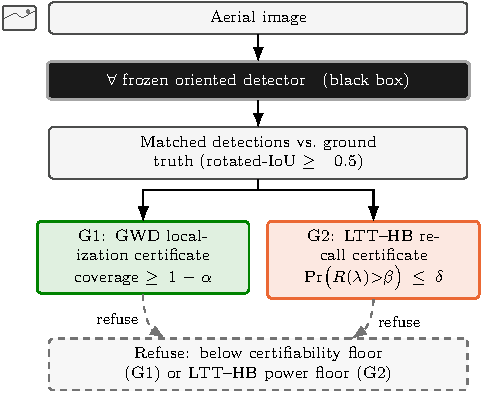
\includegraphics{../figures-src/fig0_overview.pdf}
\caption{Method overview. The wrapper treats any frozen oriented detector as a black box (five
architectures certified in this paper: RTMDet-R-l, Oriented R-CNN, RoI Transformer, S2A-Net, plus the
Config-A DOTA detector-zoo arm). Matched detections feed two independent, coupled certificates: G1
Mondrian (per-class) GWD calibration, giving a certified GWD-ball region at coverage $\ge 1-\alpha$; and
G2, a Learn-then-Test Hoeffding--Bentkus (LTT--HB) certified rotated-IoU recall bound. Either branch
refuses --- rather than reports --- on strata that do not clear its own certifiability floor
($\alpha_{\min}=1/(n_{\mathrm{cal}}+1)>\alpha$ for G1; below the LTT--HB power floor for
G2).}\label{fig:overview}
\end{figure}

\section{Related Work}\label{sec:related}
\textbf{Conformal and risk-controlled object detection.} Split conformal prediction \citep{vovk2005algorithmic}
and its Mondrian (group-conditional) variant \citep{vovk2003mondrian} give finite-sample marginal coverage
under exchangeability; adaptive, heteroscedasticity-aware conformal regression \citep{romano2019cqr} is the
broader motivation for conditioning on an informative stratum (class, here) rather than reporting one
constant-width interval. For detection specifically, coordinate/corner-wise interval constructions and two-step
uncertainty calibration \citep{andeol2023conformal,timans2024twostep,ries2026probabilistic}, and conformal
risk control / sequential risk control for recall-type risks \citep{angelopoulos2022crc,andeol2025seqcrc},
target axis-aligned boxes. Learn-then-Test \citep{angelopoulos2021ltt} provides high-probability risk
certificates via multiple testing over a threshold grid, which we adopt for G2 -- itself a multiple-testing
instance of the more general risk-controlling-prediction-sets framework \citep{bates2021rcps}. Distribution-free
structured-output UQ has also been built for other per-location targets, notably pixel-wise image-to-image
regression \citep{angelopoulos2022im2im}, but not, to our knowledge, for the periodic, seam-discontinuous
angle parameter of an oriented box. The one aerial treatment we
are aware of \citep{copley2024copa} conformalizes an axis-aligned YOLO detector.

\textbf{Oriented detection with conformal guarantees (the closest neighbour).} The most adjacent system,
EAV-DETR \citep{eavdetr2026}, couples arbitrary-view oriented UAV detection with a ``Pose-Aware
Mondrian Conformal Prediction'' (PA-MCP) module that uses the UAV flight pose as the Mondrian stratum
to produce conditional-coverage prediction sets. Its contribution is a single, bespoke high-accuracy detector:
EAV-DETR is a real-time oriented-DETR variant whose gains come from two trained architectural
components (scale-adaptive center supervision and anisotropic decoupled rotational attention), evaluated on
two UAV benchmarks (CODrone, UAV-ROD), with the conformal layer calibrated on top of that detector and
conditioned on a platform-specific pose prior. Our contribution is orthogonal and complementary: a
detector-agnostic, purely post-hoc certification wrapper that treats any frozen detector as a
black box --- five detector architectures across three satellite/aerial benchmarks --- strata on object
class rather than on capture pose (so it needs no platform metadata), and adds machinery a single built-in
guarantee does not carry: explicit certifiability-floor refusals, a coupled certified-recall guarantee
via Learn-then-Test \citep{angelopoulos2021ltt}, and out-of-sample coverage validation. The two lines
therefore complement rather than compete --- a purpose-built UAV detector with an integrated pose-conditioned
set, versus a reusable geometry-certification layer for the frozen detectors practitioners already deploy.
(The differentiation here rests on EAV-DETR's public abstract and code release; the full text is paywalled.)

\textbf{Uncertainty quantification in the remote-sensing venues.} Uncertainty-aware and evidential models are
by now an established genre in the remote-sensing literature --- e.g.\ uncertainty-aware building extraction
\citep{uanet2024}, evidential open-set hyperspectral classification \citep{ssel2024}, and Bayesian
uncertainty for explainable SAR target detection \citep{huang2023sarunc} --- but these report
heuristic or Bayesian uncertainty scores, not finite-sample coverage guarantees. We instead bring
distribution-free, finite-sample conformal and risk-control guarantees to oriented detection in that setting.

\textbf{Calibration of object detectors.} A separate, longer-standing line recalibrates detector confidence
scores post hoc, from classifier temperature scaling \citep{guo2017calibration} to box-location/scale-conditional
calibration for detection specifically \citep{kuppers2020multivariate} and calibration under domain shift
\citep{munir2022calibration}. Calibration reduces the average miscalibration of a score but carries no
finite-sample coverage guarantee for any individual stratum; G1 and G2 instead certify --- and explicitly
refuse below their respective certifiability/power floors rather than report a miscalibrated number.

\textbf{Oriented detection and the angle representation.} DOTA \citep{xia2018dota,ding2021dotabench} and
DIOR-R \citep{cheng2022diorr} are the standard oriented benchmarks, with HRSC2016 \citep{liu2017hrsc2016}
(used here as the elongation-dominated HRSC2016-MS arm, \S\ref{sec:configA}) and FAIR1M \citep{sun2022fair1m}
the adjacent fine-grained oriented benchmarks we do not certify on. The five architectures our wrapper
certifies span the major design lineages of oriented detection: two-stage RoI-warping (RoI Transformer
\citep{ding2019roitrans}, Oriented R-CNN \citep{xie2021orcnn}), single-stage feature alignment (S2A-Net
\citep{han2022s2anet}, RTMDet-R \citep{lyu2022rtmdet}), and point-based representation (Oriented RepPoints
\citep{li2022reppoints}, a Config-A zoo detector); the broader lineage these descend from includes the
earliest rotated-anchor proposal networks \citep{ma2018rrpn}, vertex-regression \citep{xu2021glidingvertex},
progressive refinement \citep{yang2021r3det}, rotation-equivariant \citep{han2021redet}, and attention-based
small/cluttered-object \citep{yang2019scrdet} designs --- our wrapper is agnostic to which of these a
practitioner deploys, treating each as a frozen black box. All in-house training uses the MMRotate toolbox
\citep{zhou2022mmrotate}. Gaussian-distance losses (GWD \citep{yang2021gwd}, KLD \citep{yang2021kld}) replace
discontinuous angle regression with a smooth distance between box-induced Gaussians; we reuse that
representation as a conformal score, not a loss.

\section{Methods}\label{sec:methods}
\textbf{The GWD nonconformity score.} We canonicalize every ingested box to the \texttt{le90} long-edge
convention ($w\ge h$, $\theta\in[-\tfrac{\pi}{2},\tfrac{\pi}{2})$) and represent it as a $2$-D Gaussian
$\mathcal{N}(\mu,\Sigma)$ with $\mu=(cx,cy)$ and $\Sigma = R(\theta)\,\mathrm{diag}((w/2)^2,(h/2)^2)\,
R(\theta)^\top$. $\Sigma$ is a smooth function of $(w,h,\theta)$ with no seam discontinuity and no
square degeneracy (as $w\to h$, $\Sigma$ becomes isotropic and the ill-defined orientation is absorbed). The
nonconformity between a prediction $\hat p$ and a ground-truth box $g$ is the $2$-Wasserstein (GWD) distance
\[
s(\hat p, g)^2 = \lVert \hat\mu-\mu \rVert^2 + \mathrm{Tr}\!\Big(\hat\Sigma+\Sigma-2\big(\hat\Sigma^{1/2}
\Sigma\,\hat\Sigma^{1/2}\big)^{1/2}\Big),
\]
with the closed-form $2\times 2$ Bures term; an optional scale normalization $s/\sqrt{\hat w \hat h}$ is
preregistered and ablated.

\begin{figure}[t]\centering
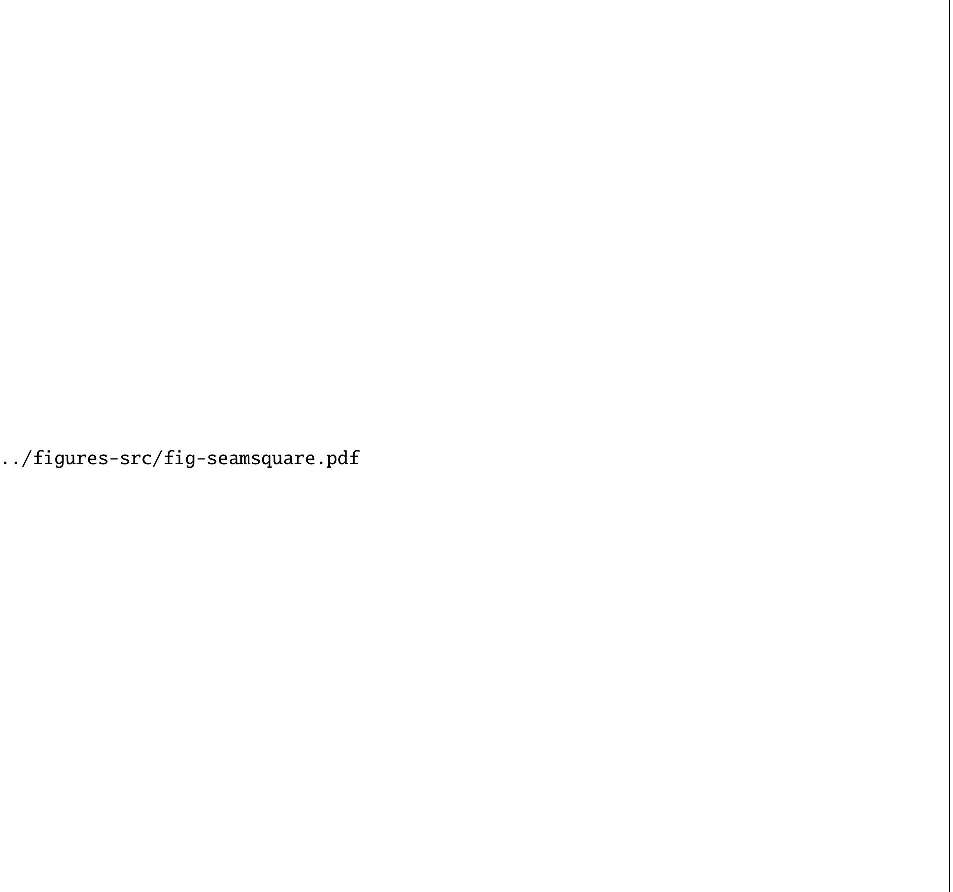
\includegraphics[width=0.98\linewidth]{../figures-src/fig-seamsquare.pdf}
\caption{Why the nonconformity score is a Wasserstein distance, not a coordinate gap (all GWD values
computed with the released \texttt{rotcert} implementation). (a)~A prediction at $\theta_{\mathrm{pred}}=-88^\circ$
and the ground truth at $+88^\circ$ are $176^\circ$ apart coordinate-wise but describe nearly the
same box; the GWD assigns $0.13$\,px. (b)~For a square box the long-edge angle is unidentifiable: the
identical box at $\theta=0^\circ$ and $\theta=90^\circ$ is charged $90^\circ$ by a coordinate-wise
score and exactly $0$ by GWD. (c)~Sweeping the prediction angle with the ground truth fixed at
$+88^\circ$: the raw coordinate gap spans $0$--$178^\circ$ (and jumps at the wrap), while GWD stays
small and smooth through the seam --- a score whose spurious range is a hundred times its
informative range forces vacuously wide conformal intervals. (d)~The same argument measured,
not argued: per-class certified radius ratio (GWD $\div$ best baseline) across the $180$
non-degenerate class cells of the family --- GWD is smaller in $91/180$ (with the three
CI-excluding-zero cells marked in Figure~\ref{fig:covmatched}d and none surviving Holm).}
\label{fig:seamsquare}
\end{figure}

\textbf{What the GWD-ball certifies, made actionable.} The G1 region is a ball in the GWD metric:
$S(\hat p)=\{b: s(\hat p,b)\le\hat q\}$ certifies, with probability $\ge 1-\alpha$, that the true box lies
within GWD distance $\hat q$ of the prediction. Because $s^2=\lVert\hat\mu-\mu\rVert^2+\mathrm{Bures}^2(\hat\Sigma,\Sigma)$
is a sum of two non-negative terms, the ball is \emph{contained in} the center slab
$\{b:\lVert\hat\mu-\mu\rVert\le\hat q\}$, so the same certificate implies --- with no loss of coverage, by
monotonicity of probability under set inclusion --- that the true object center lies within $\hat q$ pixels of
the prediction: a directly usable localization radius (\S\ref{sec:actionable}). GWD is not rotated-IoU:
distance in Gaussian-Wasserstein space is monotonically related to, but not a calibrated function of, box
overlap, so the ball is not an IoU level-set and must not be read as ``the true box is at IoU $\ge x$'';
but a user who wants that guarantee obtains it by conformalizing a $1-$rotated-IoU score directly, which we
promote from an ablation to a reported per-class \emph{certified IoU floor} (\S\ref{sec:actionable}). GWD
remains the primary score because it is simultaneously seam-continuous, square-safe, and closed-form; the
per-parameter envelope we report for visualization (a bounding box on $cx,cy,w,h$ and an arc on $\theta$)
remains a conservative outer approximation and its per-axis widths are not calibrated marginal intervals.

\textbf{G1 --- per-detection coverage regions, measured out-of-sample.} Given matched calibration pairs, let
$\hat q$ be the $\lceil(1-\alpha)(n_{\mathrm{cal}}+1)\rceil/n_{\mathrm{cal}}$ empirical quantile of the scores.
We calibrate per class (Mondrian, group $=$ class) and refuse any stratum whose certifiability floor
$\alpha_{\min}=1/(n_{\mathrm{cal}}+1)$ exceeds $\alpha$. Coverage is evaluated out-of-sample: over
$R{=}20$ repeated scene-level splits (calibration $40\%$ / matching $20\%$ / held-out evaluation $40\%$,
% split implementation: rotcert/splits.py
split-seed $=$ repeat index), we fit $\hat q$ on the calibration scenes and measure
coverage on the disjoint evaluation scenes, reporting the across-repeat mean and a BCa $95\%$ CI.

\textbf{G1 is conditional on detection.} It certifies localization given a true positive at the
operating rotated-IoU; missed detections and false positives are the job of G2.

\textbf{G2 --- certified rotated-IoU recall / FNR.} Retaining detections with confidence $\ge\lambda$, define
the per-image risk $R(\lambda)=$ mean miss rate, monotone in $\lambda$. We select $\lambda$ by Learn-then-Test
Hoeffding--Bentkus over a $\lambda$-grid controlling $\Pr(R(\lambda)>\beta)\le\delta$. The exchangeable unit is
the image, so per-class certification is limited by class-bearing images, not instances. Below the
LTT-HB power floor ($n_{\mathrm{img}}\gtrsim\ln(G/\delta)/(2(\beta-\hat R)^2)$, Bentkus-tightened) the tool
refuses and prints the floor.

\textbf{Baselines and the head-to-head.} The same pipeline runs comparison scores through one interface: naive
coordinate-wise CP with per-coordinate Bonferroni (B1, the canonical corner-wise conformal
object-detection baseline \citep{degrancey2022}), axis-aligned-hull CP (B2), and wrapped-geodesic,
doubled-angle, $1-$rotated-IoU ablations. We report the regime-conditional coverage of B1 in
\S\ref{sec:results} (descriptive). The preregistered efficiency head-to-head (class-blocked bootstrap,
Holm-corrected across baseline $\times$ detector $\times$ dataset) ran under the signed freeze and is reported
in \S\ref{sec:holm8}, where GWD is smaller in all $8$ of $8$ cells but is reported as a preregistered
descriptive outcome (the single-split test is degenerate; see the disclosure there).
% source: holm8_2026-07-12/holm8_result.json (8/8 cells GWD smaller; single-split p degenerate at 1/2001 floor)

\textbf{Threats: an in-sample audit defect, found and corrected.} An earlier pilot pipeline
% defect site: next_boot_rotcert.sh reused the same matched.jsonl for calibrate and audit
passed the same matched detection--ground-truth records to both the calibration and audit steps, so
the coverage it reported was the split-conformal calibration-set coverage
$\lceil(1-\alpha)(n+1)\rceil/n$ --- for the DOTA pilot, $48{,}719/54{,}131=0.90002$, which reproduces that
in-sample identity exactly and the nominal target to $\approx4$ significant figures ($0.9000$). That number is
an algebraic identity, independent of the score: any nonconformity
function (GWD, naive, or noise) yields it, so it has zero power to validate GWD. We correct this by
reporting the out-of-sample $R{=}20$ number throughout (\S\ref{sec:results}); the in-sample value is retained
only as a labelled self-consistency diagnostic, never as validation. This is disclosed here rather than left
for a reader to infer.

\textbf{Scene-level discipline.} DOTA is tiled into overlapping $1024\times1024$ crops, so one object appears
in adjacent crops; all splitting is at the level of the source scene (never the crop), and every
coverage CI is scene-clustered. The out-of-sample $R{=}20$ protocol also probes the box-level exchangeability
approximation: because each repeat is an independent scene-level partition, the spread of the $20$ per-repeat
coverages (reported as min/max) is a direct check that the point estimate is stable under scene re-partition,
not merely that its CI is wide.

\section{Experimental Setup}\label{sec:setup}
DOTA-v1.0 pilot. We certify RTMDet-R-l (frozen Apache-2.0 MMRotate \citep{zhou2022mmrotate} zoo checkpoint) on the DOTA-v1.0
\citep{xia2018dota} validation split ($15$ classes); calibration and evaluation use val only (the test server
is untouched). Boxes are canonicalized to \texttt{le90}; matching is greedy one-to-one at rotated-IoU $\ge
0.5$ within class. Levels are $\alpha=0.10$ (G1) and $(\beta,\delta)=(0.20,0.05)$ (G2). G1 coverage is the
out-of-sample $R{=}20$ scene-split number.

\textbf{DIOR-R extension.} No license-clean DIOR-R-trained checkpoint exists, so both detectors (Oriented
R-CNN R-50, RTMDet-R-l) are trained in house on DIOR-R \citep{cheng2022diorr} trainval via Apache-2.0
mmrotate; certification runs on the DIOR-R test split ($11{,}738$ images; single-tile, scene $=$ image) under
the identical protocol. Training setup. Oriented R-CNN is trained $1\times$ ($12$ epochs) with AdamW
% training provenance: dior_train_results_2026-07-10/.../orcnn_dior/.../oriented-rcnn-le90_r50_fpn_1x_dior.py
($\mathrm{lr}=10^{-4}$, weight decay $0.05$) rather than the config-default SGD, together with an
 annotation-filtering step that drops degenerate zero-area DIOR-R ground-truth boxes
 (removing boxes below a minimum width or height, and images left with no valid ground truth); both changes were made after those boxes destabilized the
default recipe. RTMDet-R-l is trained $3\times$ ($36$ epochs). Checkpoints are saved at the $12$-epoch interval
with no best-checkpoint hook, so each detector is deployed at the final epoch of its fixed schedule.
For RTMDet-R-l the intermediate epoch-$24$ checkpoint scored higher on the test split ($69.65$) than the
% source: dior_train_results_2026-07-10 rtmdet_r_dior seed_0 scalars.json (epoch 24 dota/mAP 0.6965, epoch 36 0.6836)
deployed epoch-$36$ ($68.36$); because the validation loop evaluated on that same test split, selecting
epoch $24$ would be checkpoint selection on the evaluation set, so we deploy the final epoch and report the
lower number rather than adopt the higher one.

mAP reproduction (AOPG gate, preregistered K3), executed post-freeze. The in-house detectors reproduce
DIOR-R test-split mAP of $62.61$ (Oriented R-CNN, $1\times$) and $68.36$ (RTMDet-R-l, $3\times$), against the
AOPG published DIOR-R reference of $64.41$ \citep{cheng2022diorr}. The AOPG table lists neither detector as a
same-method row, so its $\pm0.5$ identity-reproduction tolerance cannot be met by construction ($-1.80$,
$+3.95$ vs.\ AOPG). A same-method external anchor does exist: a recent benchmark table reports Oriented R-CNN
R-50 at $64.30$ mAP on DIOR-R \citep{ding2026rtoriented} --- essentially AOPG's $64.41$ and within $1.7$ points
of our $1\times$ reproduction ($62.61$); the DIOR-R tables that state a schedule use $12$ epochs ($1\times$),
matching ours. We could not verify any same-method Oriented R-CNN figure near the $67$--$68$ leaderboard
band a naive comparison invites: that band is recent end-to-end transformer detectors, not Oriented R-CNN.
Both reproduced scores fall in the published DIOR-R band (Oriented R-CNN between Gliding Vertex and RoI
Transformer at $1\times$; RTMDet-R-l above the entire 2021 table). We disclose the gap rather than chase it,
and certification uses reproduced scores only, never paper-quoted ones.

\section{Results}\label{sec:results}
\subsection{G1 --- out-of-sample localization coverage across the four original cells}
% source: pilot_oos_2026-07-11/dota_r20_coverage.json; dior_cert_results_2026-07-11/{orcnn,orcnn_fixedgt,rtmdet}/r20_coverage.json (marginal_coverage_across_repeats)
The GWD certificate's held-out coverage is at nominal on both DIOR-R cells and $\approx1$--$1.2$ points below
on both DOTA cells (Table~\ref{tab:g1oos}). Decisively, the full detector$\times$dataset cross now exists:
both detector families cover at nominal on DIOR-R ($0.9004$/$0.9012$) and below on DOTA
($0.8902$/$0.8879$) --- the shortfall appears to be a dataset artifact --- DOTA's
overlapping $1024$-px crops leave residual within-scene correlation that scene-level splitting reduces but does
not remove --- not a detector or score defect. The in-sample audit (Table~\ref{tab:g1oos}, right column) is a
labelled diagnostic only (see Methods/Threats): it equals $0.900$ by construction for any score.

\begin{table}[t]\centering\small
\caption{G1 marginal coverage, out-of-sample $R{=}20$ scene-split (BCa $95\%$ CI; nominal $0.90$).
The in-sample column is the tautological self-consistency value ($\lceil(1-\alpha)(n+1)\rceil/n$), kept as a
diagnostic only. From the frozen out-of-sample coverage records.}\label{tab:g1oos}
% source dirs: pilot_oos_2026-07-11/ and dior_cert_results_2026-07-11/
\begin{tabular}{llcc}
\toprule
Cell & detector $\cdot$ dataset & OOS $R{=}20$ coverage & in-sample (diag.) \\
\midrule
DOTA pilot          & RTMDet-R-l $\cdot$ DOTA   & $0.8879$ $[0.8774,0.8979]$ & $0.900$ \\
% source: orcnn_dota_cert_2026-07-11/r20_coverage.json (published mmrotate ckpt 57c88621, same val tiles as pilot)
DOTA-ORCNN          & Oriented R-CNN $\cdot$ DOTA & $0.8902$ $[0.8780,0.8995]$ & $0.900$ \\
DIOR-ORCNN          & Oriented R-CNN $\cdot$ DIOR-R & $0.9004$ $[0.8987,0.9020]$ & $0.900$ \\
DIOR-RTMDet         & RTMDet-R-l $\cdot$ DIOR-R & $0.9012$ $[0.8995,0.9030]$ & $0.900$ \\
\bottomrule
\end{tabular}
\end{table}

\subsection{G1 --- per-class Mondrian certificates (all classes certified, none refused)}
% source: dior_cert_results_2026-07-11/{orcnn_fixedgt,rtmdet}/cert_gwd.json (20 strata, refused []); pilot cert_gwd.json (15 strata)
The Mondrian calibration certifies every class with $0$ refused in every cell: $15/15$ on DOTA and
$20/20$ on DIOR-R for both Oriented R-CNN and RTMDet-R-l. Table~\ref{tab:g1mondrian} lists the DOTA pilot's
per-class GWD-ball radii, spanning nearly two orders of magnitude (compact ships/vehicles tightest;
elongated ground-track-field/harbor widest); the DIOR-R rosters show the same compact-vs-infrastructure spread
(e.g.\ DIOR ship $\hat q{=}3.99$, area $50$\,px$^2$; dam $\hat q{=}73.9$, area $17{,}134$\,px$^2$).

\textbf{A recovered-classes provenance note (DIOR-R).} The first DIOR-R Oriented R-CNN run certified $18/20$
classes: two multi-word classes (expressway-service-area and expressway-toll-station) were
excluded because the detector dump lower-cased them while the ground truth capitalized them, so the
class-exact matcher found $0$ true positives --- the tool correctly excluded-and-counted them. Re-running
against a casing-normalized ground truth recovers both ($20/20$) and leaves the other $18$ classes'
per-class $\hat q$ and $n_{\mathrm{cal}}$ bit-identical (verified class-by-class), and out-of-sample
coverage unchanged ($0.9001\!\to\!0.9004$) --- a surgical fix that also demonstrates the refusal machinery
behaving as designed on a real label-hygiene fault.

\begin{table}[t]\centering\small
\caption{G1 per-class GWD certificates on the DOTA-v1.0 pilot ($\alpha=0.10$). $\hat q$ is the GWD-ball
radius; area is the $(cx,cy)$ coverage-slice area $\pi\hat q^2$ (px$^2$). All $15$ classes certified, $0$
refused. From the frozen per-class certification record.}\label{tab:g1mondrian}
% source: pilot_results_2026-07-10/.../cert_gwd.json
\begin{tabular}{lccc}
\toprule
Class & $n_{\mathrm{cal}}$ & $\hat q$ & Area (px$^2$) \\
\midrule
% source: cert_gwd.json strata.*.calibrator.q_hat / n_cal / set_size_cxcy (verified 2026-07-11)
ship               & 18{,}125 & 3.50 & 38.6 \\
small-vehicle      & 10{,}394 & 3.14 & 30.9 \\
large-vehicle      & 8{,}727  & 3.73 & 43.7 \\
storage-tank       & 4{,}291  & 2.80 & 24.6 \\
plane              & 4{,}299  & 7.48 & 175.6 \\
harbor             & 4{,}007  & 19.14 & 1{,}151.0 \\
tennis-court       & 1{,}510  & 2.97 & 27.8 \\
bridge             & 681      & 9.34 & 274.3 \\
swimming-pool      & 660      & 6.59 & 136.3 \\
baseball-diamond   & 347      & 10.30 & 333.1 \\
basketball-court   & 266      & 6.37 & 127.4 \\
roundabout         & 262      & 5.55 & 96.8 \\
soccer-ball-field  & 238      & 17.52 & 963.9 \\
ground-track-field & 205      & 22.09 & 1{,}533.1 \\
helicopter         & 119      & 12.01 & 452.9 \\
\bottomrule
\end{tabular}
\end{table}

\textbf{Per-class conditional coverage on the 20-class dataset (post-hoc, descriptive).} A hostile reviewer
may ask whether the Mondrian certificate merely holds marginally while hiding per-class shortfalls. It
does not. Mirroring the shipped Mondrian machinery (grouping on object class) under the same
$R{=}20$ scene-split protocol, we measure the out-of-sample coverage of the per-class GWD certificate
within each of the $20$ DIOR-R classes (Table~\ref{tab:diorperclass}). Every class clears the G1
certifiability floor $\alpha_{\min}{=}1/(n_{\mathrm{cal}}{+}1)\!<\!\alpha$ ($0/20$ refused; the smallest
class, dam, has $n_{\mathrm{cal}}{=}266$), and per-class conditional coverage is tightly clustered around
nominal: pooled per-class coverage is $0.900$ in both cells, and no class deviates more than
$\approx1.3$ points from $0.90$ (Oriented R-CNN range $0.887$ golffield -- $0.913$ dam; RTMDet-R-l range
$0.891$ stadium -- $0.907$ tenniscourt), with the sub-nominal classes inside one split-to-split standard
deviation of $0.90$. The certifiability floor that does bite is the recall certificate's (G2)
images-per-class power floor, not the localization certificate: the small classes it refuses ($15/20$ for
Oriented R-CNN, $14/20$ for RTMDet-R-l --- last column) are still localization-certified at G1 with coverage
at nominal. The geometry certificate thus covers every class approximately at nominal (within
$\approx1.3$ points, one split-to-split std, of every sub-nominal class), while the recall certificate
honestly abstains on the rare ones.

\begin{table}[t]\centering\small
\caption{Per-class out-of-sample conditional coverage of the GWD certificate on the two core DIOR-R cells
($\alpha=0.10$, nominal $0.90$; $R{=}20$ scene splits, mean over repeats). $n_{\mathrm{cal}}$ is the Oriented
R-CNN full-data per-class calibration count (RTMDet-R-l counts are within a few percent). G2 recall: \texttt{O}$=$certified for Oriented R-CNN, \texttt{R}$=$certified for
RTMDet-R-l, \textemdash{}$=$refused by the LTT-HB power floor. Post-hoc / descriptive; from the frozen per-class conditional-coverage record.}\label{tab:diorperclass}
% source: dior_perclass_2026-07-15/results.json (perclass_conditional_coverage.py, R=20 Mondrian per-class OOS)
\begin{tabular}{lcccc}
\toprule
Class & $n_{\mathrm{cal}}$ & ORCNN cov. & RTMDet cov. & G2 recall \\
\midrule
ship                    & 30{,}731 & 0.899 & 0.899 & \textemdash \\
storagetank             & 16{,}081 & 0.900 & 0.900 & R \\
vehicle                 & 12{,}958 & 0.904 & 0.899 & \textemdash \\
tenniscourt             & 6{,}498  & 0.897 & 0.907 & O,R \\
airplane                & 5{,}589  & 0.898 & 0.900 & \textemdash \\
baseballfield           & 2{,}617  & 0.901 & 0.898 & R \\
windmill                & 2{,}291  & 0.900 & 0.895 & \textemdash \\
basketballcourt         & 1{,}928  & 0.898 & 0.894 & O,R \\
groundtrackfield        & 1{,}773  & 0.903 & 0.905 & O,R \\
harbor                  & 1{,}692  & 0.901 & 0.899 & \textemdash \\
bridge                  & 1{,}470  & 0.906 & 0.902 & \textemdash \\
overpass                & 1{,}183  & 0.898 & 0.895 & \textemdash \\
expressway-service-area & 962      & 0.896 & 0.905 & O,R \\
chimney                 & 808      & 0.899 & 0.900 & \textemdash \\
stadium                 & 600      & 0.906 & 0.891 & O \\
expressway-toll-station & 508      & 0.913 & 0.898 & \textemdash \\
golffield               & 459      & 0.887 & 0.899 & \textemdash \\
airport                 & 357      & 0.906 & 0.896 & \textemdash \\
trainstation            & 354      & 0.902 & 0.899 & \textemdash \\
dam                     & 266      & 0.913 & 0.903 & \textemdash \\
\bottomrule
\end{tabular}
\end{table}

\subsection{G1 --- the certificate made actionable: center-offset, orientation, and IoU-floor readouts}\label{sec:actionable}
% source: actionable_cert_2026-07-16/results.json (script/actionable_cert.py; per-class q_hat reproduced bit-for-bit from the frozen cert_gwd.json, max|q_hat - frozen| = 0 in all three cells)
A GWD-ball radius is not, on its face, a quantity a remote-sensing practitioner can act on. We therefore
translate each frozen per-class $\hat q$ --- re-derived here from the frozen matched records and gated
bit-for-bit against the certification record ($\max|\hat q-\hat q_{\mathrm{frozen}}|{=}0$ across all three
cells) --- into three interpretable geometric readouts, changing no certified number
(Table~\ref{tab:actionable}).

\emph{(i) A certified center-offset radius.} Since $s^2=\lVert\Delta\mu\rVert^2+\mathrm{Bures}^2\ge
\lVert\Delta\mu\rVert^2$, the event $\{s\le\hat q\}$ implies $\lVert\Delta\mu\rVert\le\hat q$: the GWD-ball
lies inside the center slab of half-width $\hat q$, so $\Pr(\lVert\Delta\mu\rVert\le\hat q)\ge\Pr(s\le\hat q)
\ge1-\alpha$. The center bound therefore \emph{inherits} the coverage guarantee exactly --- it is a
consequence, not an approximation. On the DOTA pilot the true center lies within $2.8$--$3.7$\,px of the
prediction for compact ships and vehicles (up to $22$\,px for the largest infrastructure classes), each with
probability $\ge0.90$.

\emph{(ii) A certified orientation half-extent.} Restricted to the pure-rotation axis through the prediction
(fixed center and size), $s^2=\mathrm{Bures}^2(\Delta\theta)$ is monotone in $|\Delta\theta|$ on
$[0,\tfrac{\pi}{2}]$, so the ball admits rotations up to $\Delta\theta_{\max}$ where
$\mathrm{Bures}(\Delta\theta_{\max})=\hat q$ at the class's median box shape. This resolution is tight exactly
where orientation is meaningful (large-vehicle $6.6^\circ$, tennis-court $2.9^\circ$, ship $11.1^\circ$) and
correctly \emph{unconstrained} ($90^\circ$) for the three near-square classes (storage-tank,
baseball-diamond, roundabout; aspect ratio $\le1.05$) whose orientation is genuinely unidentifiable --- the
square-safety of GWD rendered as an actionable output rather than a caveat. It is an outer envelope (a joint
size-and-angle error can also spend the Bures budget), reported as orientation resolution, not a marginal
interval.

\begin{figure}[t]\centering
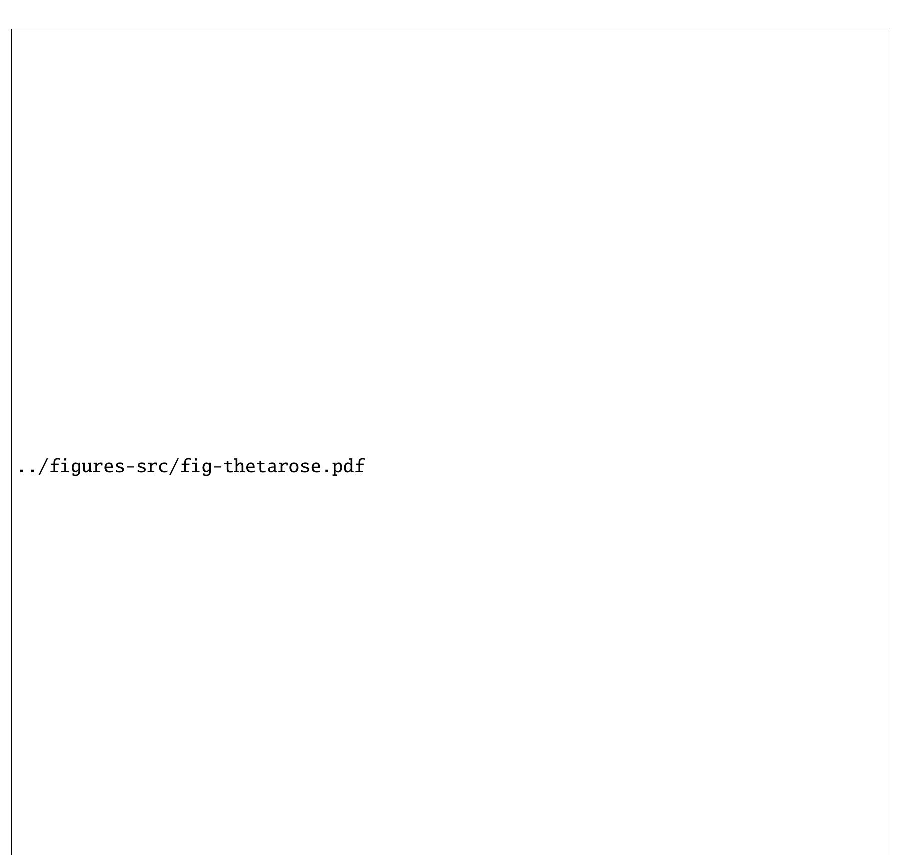
\includegraphics[width=0.9\linewidth]{../figures-src/fig-thetarose.pdf}
\caption{Per-class orientation distributions on the DIOR-R test split (frozen ground-truth record,
angles canonicalized to the long-edge convention). Elongated classes (top row: ship, harbor,
bridge; median aspect ratio $2.9$--$4.0$) carry informative, multi-modal orientation structure ---
the certified orientation half-extent is tight there ($2.9^\circ$--$11.1^\circ$). Near-square
classes (bottom row; median aspect ratio $1.0$--$1.3$) are isotropic by construction, so a
predicted angle for them is noise rather than signal: the certificate correctly reports
$90^\circ$ (unconstrained) instead of certifying an unidentifiable quantity.}
\label{fig:thetarose}
\end{figure}

\emph{(iii) A certified rotated-IoU floor.} Conformalizing $1-$rotated-IoU per class with the identical
split-conformal estimator yields $\hat q_{\mathrm{iou}}$ and hence the directly usable guarantee
$\text{rotated-IoU}(\hat p,\text{true})\ge1-\hat q_{\mathrm{iou}}$ with probability $\ge1-\alpha$. Every DOTA
class carries a non-vacuous floor between $0.61$ and $0.90$ (Table~\ref{tab:actionable}), and this calibrated
floor tracks the empirical $5$th-percentile rotated-IoU of the boxes the GWD-ball actually accepts
class-by-class (tennis-court $0.902$ vs.\ $0.903$; ship $0.757$ vs.\ $0.742$), so the abstract GWD ball and
the direct IoU certificate agree on the ground. Promoting this construction from the ablation set to a
reported certificate answers the practitioner's ``true box at IoU $\ge y$'' question without abandoning GWD's
seam-continuity and square-safety for calibration.

\emph{Breadth.} The pattern replicates on the two Config-B DIOR-R cells ($20$ classes each): certified
center-offset radii of $3.5$--$91$\,px, non-vacuous IoU floors of $0.53$--$0.82$, and orientation
unconstrained on $4$--$5$ near-square classes per cell while tightly bounded on every elongated one (full
per-class numbers in the frozen actionable-certificate record).

\emph{A second detector family and the per-class spread.} The same readouts on the DOTA-v1.0 Oriented
RepPoints cell (Table~\ref{tab:actionable-reppoints}) show exactly the per-class differentiation the
certificate is meant to expose: plane certifies at $13.1$\,px center offset with an IoU floor of $0.72$
on $4{,}355$ calibration TPs, ground-track-field at $33.7$\,px / $0.74$ on only $42$, and ship ---
on just $12$ calibration TPs --- at $50.9$\,px / $0.55$, honestly wide rather than silently tight.
Two classes with $3$--$4$ calibration TPs are refused as vacuous instead of being reported with
unusable radii. The reproduction gate is identical ($\max|\hat q-\hat q_{\mathrm{frozen}}|{=}0$).

\begin{table}[t]\centering\small
\caption{The actionable G1 certificate on a second detector family (DOTA-v1.0, Oriented RepPoints,
$\alpha=0.10$; post-freeze addition to the actionable record, same construction and reproduction gate as
Table~\ref{tab:actionable}). The per-class spread is the point: radii track the calibration support
($n_{\mathrm{cal}}$ from $4{,}355$ down to $12$), and the two classes with $3$--$4$ TPs are refused as
vacuous ($\hat q\to\infty$). $90^\circ$: a full flip is within the certified Bures budget --- here driven
by the radius, not by near-square geometry.}\label{tab:actionable-reppoints}
% source: actionable_cert_2026-08-01/results.json -> cells[DOTA-RepPoints].classes.*
\begin{tabular}{lrrrr}
\toprule
Class & $n_{\mathrm{cal}}$ & $r_{\mathrm{center}}$ (px) & $\Delta\theta_{\max}$ & IoU floor \\
\midrule
plane              & $4{,}355$ & $13.14$ & $90^\circ$          & $0.719$ \\
harbor             & $631$     & $17.51$ & $26.4^\circ$        & $0.611$ \\
baseball-diamond   & $295$     & $20.19$ & $90^\circ$          & $0.663$ \\
swimming-pool      & $275$     & $8.04$  & $37.8^\circ$        & $0.591$ \\
ground-track-field & $42$      & $33.75$ & $32.2^\circ$        & $0.736$ \\
ship               & $12$      & $50.90$ & $90^\circ$          & $0.553$ \\
\midrule
soccer-ball-field  & $4$       & \multicolumn{3}{l}{refused: vacuous (insufficient calibration TPs)} \\
large-vehicle      & $3$       & \multicolumn{3}{l}{refused: vacuous (insufficient calibration TPs)} \\
\bottomrule
\end{tabular}
\end{table}

\begin{table}[t]\centering\small
\caption{The G1 certificate made actionable on the DOTA-v1.0 pilot ($\alpha=0.10$). Each frozen per-class
GWD radius $\hat q$ is read as a certified center-offset radius $r_{\mathrm{center}}{=}\hat q$ (px; inherits
the $\ge0.90$ coverage), an orientation half-extent $\Delta\theta_{\max}$ at the median box shape, and a
directly-conformalized rotated-IoU floor $1-\hat q_{\mathrm{iou}}$ ($\ge0.90$ coverage). $\dagger$: orientation
unconstrained (near-square, aspect ratio $\le1.05$; a full $90^\circ$ flip is within the certified Bures
budget). From the frozen actionable-certificate record; $\hat q$ reproduces the certification record
exactly.}\label{tab:actionable}
% source: actionable_cert_2026-07-16/results.json -> cells[DOTA-pilot].classes.*.{r_center_px,dtheta_max_deg,iou_floor,orientation_unconstrained}
\begin{tabular}{lrrr}
\toprule
Class & $r_{\mathrm{center}}$ (px) & $\Delta\theta_{\max}$ & IoU floor \\
\midrule
ship               & 3.50  & $11.1^\circ$          & 0.757 \\
small-vehicle      & 3.14  & $14.2^\circ$          & 0.708 \\
large-vehicle      & 3.73  & $6.6^\circ$           & 0.778 \\
storage-tank       & 2.80  & $90^\circ\,\dagger$   & 0.684 \\
plane              & 7.48  & $42.6^\circ$          & 0.808 \\
harbor             & 19.14 & $25.0^\circ$          & 0.671 \\
tennis-court       & 2.97  & $2.9^\circ$           & 0.902 \\
bridge             & 9.34  & $34.9^\circ$          & 0.613 \\
swimming-pool      & 6.59  & $31.3^\circ$          & 0.616 \\
baseball-diamond   & 10.30 & $90^\circ\,\dagger$   & 0.726 \\
basketball-court   & 6.37  & $13.2^\circ$          & 0.833 \\
roundabout         & 5.55  & $90^\circ\,\dagger$   & 0.753 \\
soccer-ball-field  & 17.52 & $24.5^\circ$          & 0.701 \\
ground-track-field & 22.09 & $26.1^\circ$          & 0.791 \\
helicopter         & 12.01 & $47.2^\circ$          & 0.686 \\
\bottomrule
\end{tabular}
\end{table}

% source: figures-src/fig_showcase.pdf, built by figures-src/make_fig_showcase.py from frozen
% configB_cells_2026-07-15/s2anet/matched.jsonl + actionable_cert_2026-07-16/results.json
\begin{figure*}[t]\centering
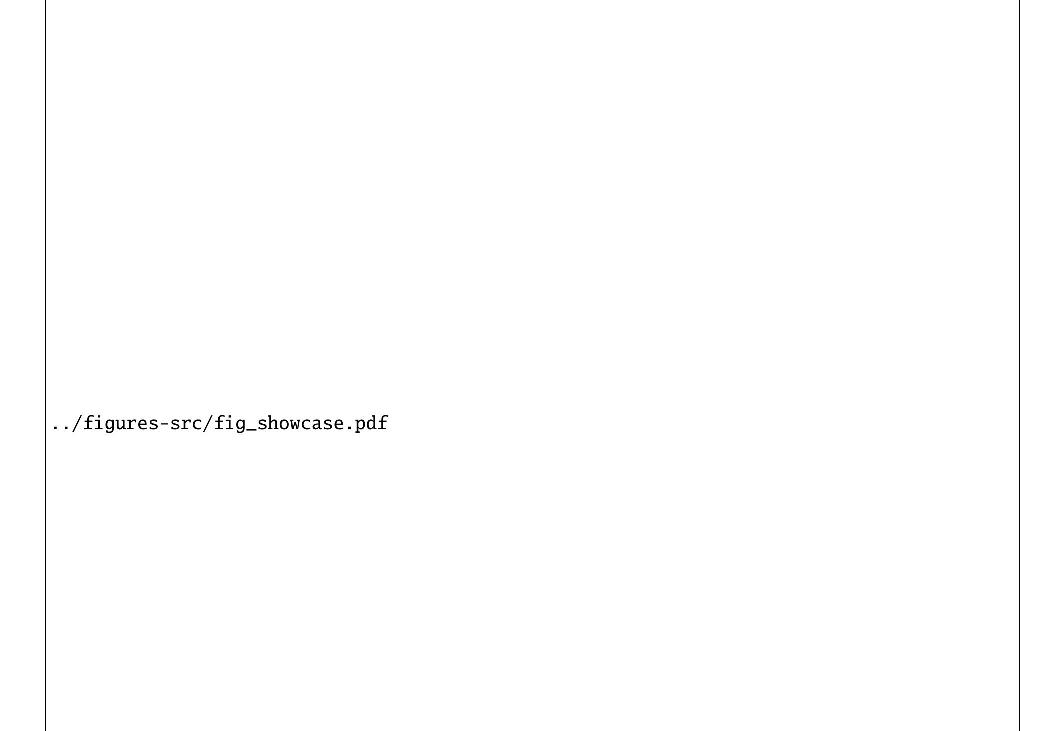
\includegraphics[width=\linewidth]{../figures-src/fig_showcase.pdf}
\caption{The G1 certificate made concrete on four DIOR-R test scenes (S2A-Net Config-B cell).
\textbf{Top row:} full scenes with matched predicted oriented bounding boxes (score $\ge0.5$).
\textbf{Bottom row:} zoom crops of one certified object per scene, showing the predicted OBB
(solid), ground truth (dashed white), the certified center-offset radius $r_{\mathrm{center}}$
(dashed circle), and the certified orientation half-extent $\Delta\theta_{\max}$ (shaded wedge;
omitted where orientation is unconstrained). The readouts are the same actionable quantities
reported in Table~\ref{tab:actionable}; the IoU floor for each class is printed in the panel label.
From the frozen actionable-certificate and matched-detection records.}\label{fig:showcase}
\end{figure*}

\subsection{G2 --- certified recall scales with images-per-class}
% source: pilot recall.json (2/15); dior_cert_results_2026-07-11/{orcnn_fixedgt,rtmdet}/recall.json (5/20, 6/20)
At $(\beta,\delta)=(0.20,0.05)$, G2 certifies a per-class FNR bound where powered and refuses
elsewhere (Table~\ref{tab:g2}, all nine cells). The certified count rises from $2/15$ on DOTA ($\sim458$ val images) to
$5/20$ and $6/20$ on DIOR-R ($11{,}738$ test images), and RTMDet-R-l (denser detections, more matched TPs)
certifies one more class than Oriented R-CNN --- direct evidence the LTT-HB power floor is data-scale
driven and moves down with more images, not a permanent ceiling. Refusals are of two honest kinds: an
infinite power floor (realized per-image miss rate $\ge\beta$, uncertifiable at any $n$; e.g.\
DIOR-ORCNN airplane, vehicle --- RTMDet's floors for the same two classes are finite ($1{,}225$ and
$75{,}149$ images, $\hat r<\beta$), refused only for insufficient images) and insufficient images
below the Bentkus floor (e.g.\ DOTA harbor $n_{\mathrm{img}}{=}112<135.7$). The tool prints the floor rather than reporting an uncertifiable number.

\begin{table}[t]\centering\small
\caption{G2 certified-recall counts across all nine cells ($\beta{=}0.20$, $\delta{=}0.05$). Certified count
scales with images-per-class: the high-image DIOR-R cells certify $5$--$7/20$, while the low-image
HRSC2016-MS ($n_{\mathrm{img}}{=}440$) and DOTA-v1.0 zoo ($n_{\mathrm{img}}{=}1093$) cells refuse at the
LTT-HB power floor. From the per-cell certification outputs.}\label{tab:g2}
% source: pilot recall.json (2/15); dior_cert_results_2026-07-11/{orcnn_fixedgt,rtmdet}/recall.json (5/20, 6/20);
% configB_cells_2026-07-15/{roi_trans,s2anet}/recall.json (5/20, 7/20);
% configA_cert_2026-07-14/{hrsc_orcnn,hrsc_rtmdet,zoo_roi_trans,zoo_oriented_reppoints}/recall.json (0/N; per_class certified counts + pooled r_hat / n_img verified 2026-07-16)
\begin{tabular}{ll>{\raggedright\arraybackslash}p{0.52\textwidth}}
\toprule
Cell & cert. / total & certified classes ($\lambda^\star$, realized risk), or refusal \\
\midrule
DOTA pilot           & $2/15$ & small-vehicle ($0.051$, $0.024$), tennis-court ($0.094$, $0.001$) \\
DIOR-R ORCNN         & $5/20$ & basketballcourt, tenniscourt, stadium, groundtrackfield, expressway-service-area \\
DIOR-R RTMDet-R-l    & $6/20$ & basketballcourt, tenniscourt, groundtrackfield, expressway-service-area, baseballfield, storagetank \\
DIOR-R RoI Transf.   & $5/20$ & basketballcourt, tenniscourt, stadium, groundtrackfield, expressway-service-area \\
DIOR-R S2A-Net       & $7/20$ & baseballfield, basketballcourt, groundtrackfield, ship, stadium, storagetank, tenniscourt \\
HRSC ORCNN           & $0/1$  & refused: LTT-HB power floor ($n_{\mathrm{img}}{=}440$, $\hat r{=}0.5464$) \\
HRSC RTMDet-R        & $0/1$  & refused: power floor ($n_{\mathrm{img}}{=}440$, $\hat r{=}0.6076$) \\
DOTA RoI Transf.     & $0/15$ & refused: power floor ($n_{\mathrm{img}}{=}1093$, $\hat r{=}0.9380$) \\
DOTA RepPoints       & $0/15$ & refused: power floor ($n_{\mathrm{img}}{=}1093$, $\hat r{=}0.8496$) \\
\bottomrule
\end{tabular}
\end{table}

\subsection{G2 made actionable: the power floor is a price tag, not a verdict}
% source: g2_planning_2026-08-01/results.json (post-freeze exploratory; closed-form inversion of the
% recorded LTT-HB Bentkus floors; recomputed floors reproduce every recorded finite floor, 113/113 cells)
The LTT--HB power floor is closed-form in the recorded quantities,
$n_{\mathrm{img}} \ge \ln(G/\delta)\,/\,(2(\beta-\hat r)^{2}\times 1.75)$, so every refusal can be
inverted into an explicit per-class planning readout (Table~\ref{tab:g2planning}). On the DIOR-ORCNN
cell the $15$ refusals split into two sharply different regimes. Six classes have a \emph{finite} floor:
golffield needs only $+261$ further images ($491\to752$), and four more classes certify for a one-to-four-fold
data increase; every finite-floor refusal also clears at a slightly looser tolerance with the data it
already has ($\beta\ge0.21$--$0.26$, last column). The remaining nine are \emph{unreachable at}
$\beta{=}0.20$: their realized per-image miss rate already exceeds $\beta$ ($\hat r$ up to $0.502$ for
dam), so no calibration budget certifies them --- the remedy is a better detector or an explicitly
looser $\beta$, and the tool says which. Table~\ref{tab:g2sweep} aggregates the same inversion across all
cells: at the frozen $(\beta,\delta)$ the cells certify $0$--$7$ classes, while relaxing to
$\beta{=}0.30$ ($0.40$) would certify $9$--$14$ ($10$--$17$) of $20$ on the DIOR-R cells --- the refusal
count is a ($\beta$, data-budget) dial the practitioner can read directly, reported descriptively.

\begin{table}[t]\centering\small
\caption{Per-class G2 planning readout, DIOR-R Oriented R-CNN ($\beta{=}0.20$, $\delta{=}0.05$; post-freeze
exploratory, descriptive). Refusals split into finite-floor (reachable with more images, or at a looser
$\beta$ with current data) and infinite-floor ($\hat r\ge\beta$: uncertifiable at any budget).
From the closed-form inversion of the frozen recall records.}\label{tab:g2planning}
% source: g2_planning_2026-08-01/results.json; rows auto-generated by g2_planning_curve.py (verification: floors reproduce frozen recall.json)
\begin{tabular}{lcccl}
\toprule
Class & $n_{\mathrm{img}}$ & $\hat r$ & power floor & planning readout \\
\midrule
groundtrackfield & --- & $0.048$ & met ($86$) & certified \\
stadium & --- & $0.089$ & met ($160$) & certified \\
basketballcourt & --- & $0.110$ & met ($244$) & certified \\
expressway-service-area & --- & $0.112$ & met ($253$) & certified \\
tenniscourt & --- & $0.137$ & met ($491$) & certified \\
\midrule
golffield & $491$ & $0.149$ & $752$ & $+261$ img / $\beta\ge0.21$ \\
windmill & $809$ & $0.167$ & $1\,762$ & $+953$ img / $\beta\ge0.22$ \\
baseballfield & $1\,311$ & $0.174$ & $2\,852$ & $+1\,541$ img / $\beta\ge0.21$ \\
ship & $1\,404$ & $0.174$ & $2\,964$ & $+1\,560$ img / $\beta\ge0.21$ \\
storagetank & $894$ & $0.177$ & $3\,666$ & $+2\,772$ img / $\beta\ge0.22$ \\
chimney & $447$ & $0.188$ & $14\,039$ & $+13\,592$ img / $\beta\ge0.26$ \\
\midrule
airplane & $705$ & $0.235$ & $\infty$ & $\beta\ge0.29$ \\
airport & $657$ & $0.461$ & $\infty$ & $\beta\ge0.52$ \\
bridge & $1\,299$ & $0.354$ & $\infty$ & $\beta\ge0.39$ \\
dam & $503$ & $0.502$ & $\infty$ & $\beta\ge0.56$ \\
expressway-toll-station & $634$ & $0.238$ & $\infty$ & $\beta\ge0.29$ \\
harbor & $813$ & $0.450$ & $\infty$ & $\beta\ge0.50$ \\
overpass & $1\,101$ & $0.277$ & $\infty$ & $\beta\ge0.32$ \\
trainstation & $501$ & $0.305$ & $\infty$ & $\beta\ge0.37$ \\
vehicle & $3\,308$ & $0.286$ & $\infty$ & $\beta\ge0.31$ \\
\bottomrule
\end{tabular}
\end{table}

\begin{table}[t]\centering\small
\caption{G2 planning summary across cells (post-freeze exploratory, descriptive): certified ($A$),
finite-floor refused ($B$), unreachable refused ($C$) at the frozen $(\beta,\delta){=}(0.20,0.05)$, and
classes certifiable with current data under looser $\beta$. From the closed-form inversion of the frozen
recall records.}\label{tab:g2sweep}
% source: g2_planning_2026-08-01/results.json; rows auto-generated by g2_planning_curve.py
\begin{tabular}{lcccccc}
\toprule
Cell & $A$/total & $B$ & $C$ & $\beta{=}0.25$ & $\beta{=}0.30$ & $\beta{=}0.40$ \\
\midrule
DOTA pilot & $2/15$ & $12$ & $1$ & $8$ & $9$ & $10$ \\
DIOR-R ORCNN & $5/20$ & $6$ & $9$ & $10$ & $13$ & $17$ \\
DIOR-R RTMDet-R-l & $6/20$ & $8$ & $6$ & $12$ & $12$ & $15$ \\
DIOR-R RoI Transf. & $5/20$ & $5$ & $10$ & $10$ & $14$ & $17$ \\
DIOR-R S2A-Net & $7/20$ & $4$ & $9$ & $10$ & $12$ & $13$ \\
HRSC ORCNN & $0/1$ & $0$ & $1$ & $0$ & $0$ & $0$ \\
HRSC RTMDet-R & $0/1$ & $0$ & $1$ & $0$ & $0$ & $0$ \\
DOTA RoI Transf. & $0/15$ & $1$ & $14$ & $0$ & $0$ & $0$ \\
DOTA RepPoints & $0/15$ & $2$ & $13$ & $0$ & $0$ & $1$ \\
\bottomrule
\end{tabular}
\end{table}

\begin{figure*}[t]\centering
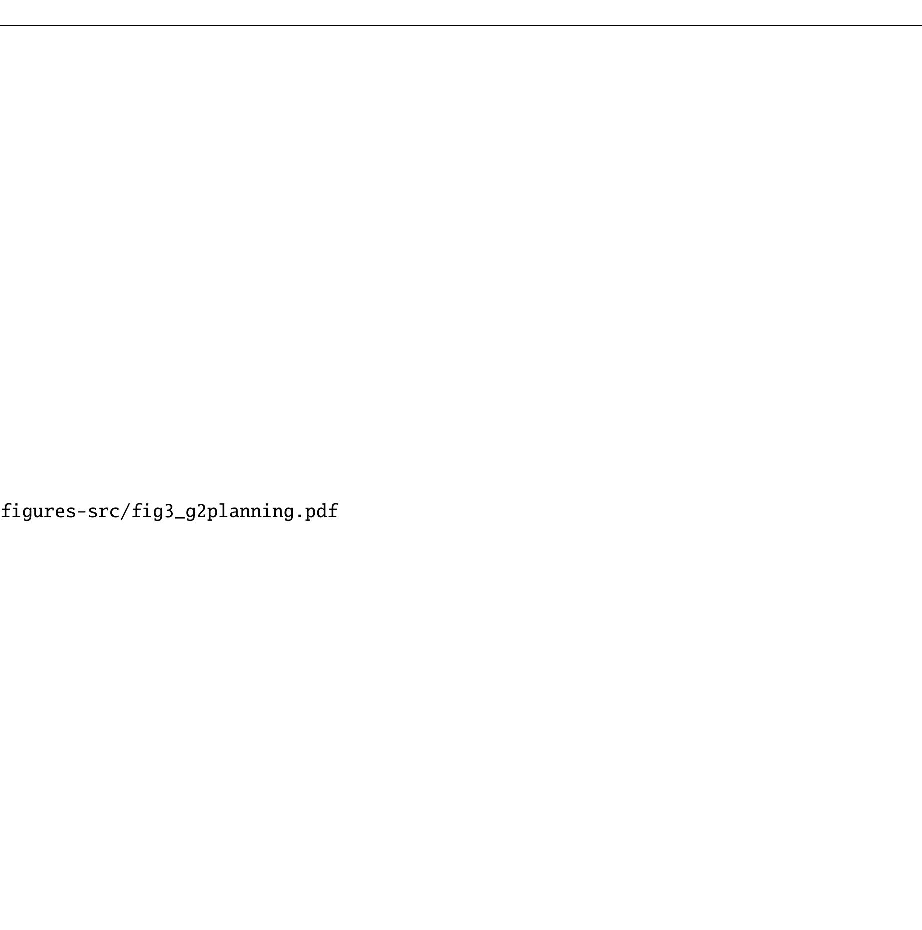
\includegraphics[width=\linewidth]{../figures-src/fig3_g2planning.pdf}
\caption{The G2 power floor as a planning readout (post-freeze exploratory; closed-form inversion
of the frozen recall records, no LTT re-run). \textbf{a:} recorded per-class calibration images
$n_{\mathrm{img}}$ vs.\ the Bentkus power floor for the refused classes (log--log; the dashed line is
``floor met''). \textbf{b:} per-cell regime split --- certified, refused with a finite (reachable)
floor, refused as unreachable ($\hat r\ge\beta$) --- across all nine cells. \textbf{c:} classes
certifiable with current data as the recall tolerance $\beta$ relaxes; the frozen operating point
$\beta{=}0.20$ is marked. \textbf{d:} distribution of the per-class $\beta_{\min}$ --- the loosest
tolerance at which each refused class would certify with the data it already has. From the frozen
recall records.}\label{fig:g2planning}
% source: g2_planning_2026-08-01/results.json (script manuscripts/figures-src/make_fig3_g2planning.py; floors reproduce frozen recall.json, verification block in results.json)
\end{figure*}

\subsection{Naive coordinate-wise CP under-covers conditionally, not universally}
% source: pilot_oos_2026-07-11/dota_audit_naive.json; dior_cert_results_2026-07-11/{orcnn_fixedgt,rtmdet}/audit_naive.json (v2_stratum_coverage)
We put the paper's motivating hook to a direct regime-conditional test (Table~\ref{tab:naive}, descriptive).
The naive coordinate-wise (Bonferroni-box) baseline over-covers marginally everywhere
($0.933$--$0.936$), as Bonferroni predicts, but its coverage is strongly regime-dependent: the seam
(boundary) or square is always its most-depressed regime relative to interior. Whether it falls below
nominal is cell-dependent --- strongly on DOTA square ($0.8405$, CI $[0.801,0.864]$ below nominal; an $11$-point
deficit vs.\ its $0.9505$ interior), marginally on DIOR-ORCNN boundary ($0.8976$), and not at all on
DIOR-RTMDet (boundary $0.9121$, still above nominal). GWD is seam/square-stable on both DIOR-R cells and
degrades least at square on the RTMDet-DOTA pilot ($\approx0.88$ vs.\ naive's $0.8405$); on the DOTA-ORCNN
cell, however, both scores show a comparable square-regime deficit (GWD $0.8612$, naive $0.8591$,
in-sample diagnostic), so GWD's square-regime advantage is itself detector-dependent on DOTA rather than
universal. We therefore state the hook as a conditional claim, and note that the
preregistered set-size head-to-head is reported in \S\ref{sec:holm8} (GWD smaller in $8/8$ cells,
reported descriptively); the regime-conditional under-coverage contrast remains descriptive here.

\begin{table}[t]\centering\small
\caption{Angle-regime coverage of the naive coordinate-wise baseline vs.\ GWD (in-sample audit, nominal
$0.90$; descriptive). Naive over-covers marginally but dips below nominal only in some cells. Extended to all
four DIOR-R cells (RoI Transformer, S2A-Net added, \S\ref{sec:configB}). From the
frozen regime-audit records.}\label{tab:naive}
% source: per-cell audit_naive.json / audit_gwd.json; RoI-Trans/S2A-Net rows from configB_cells_2026-07-15/{roi_trans,s2anet}/{audit_naive.json,audit_gwd.json}
\begin{tabular}{lccccc}
\toprule
Cell & naive marg. & naive interior & naive boundary & naive square & GWD (int/bnd/sq) \\
\midrule
DOTA pilot        & $0.933$ & $0.951$ & $0.919$ & $0.841$ & $0.893/0.937/0.880$ \\
DIOR-ORCNN        & $0.935$ & $0.944$ & $0.898$ & $0.962$ & $0.886/0.910/0.933$ \\
DIOR-RTMDet       & $0.935$ & $0.945$ & $0.912$ & $0.940$ & $0.885/0.917/0.927$ \\
DIOR-RoI-Trans    & $0.936$ & $0.945$ & $0.902$ & $0.960$ & $0.885/0.910/0.934$ \\
DIOR-S2ANet       & $0.935$ & $0.944$ & $0.867$ & $0.988$ & $0.884/0.911/0.951$ \\
\bottomrule
\end{tabular}
\end{table}

\textbf{The Config-B DIOR-R extension is regime-consistent for RoI Transformer but not for S2A-Net.}
% source: configB_cells_2026-07-15/{roi_trans,s2anet}/{audit_naive.json,audit_gwd.json} (v2_stratum_coverage)
Repeating this audit on the two Config-B DIOR-R cells (\S\ref{sec:configB}) extends the table to all four
DIOR-R detectors. RoI Transformer matches the established DIOR-R pattern (boundary $0.902$, at nominal, not
below it, like DIOR-RTMDet). S2A-Net does not: its boundary coverage ($0.867$) is the only DIOR-R regime cell
in the study that dips clearly below nominal --- deeper than DIOR-ORCNN's marginal dip ($0.898$) and unlike
DIOR-RTMDet or RoI Transformer, both of which sit at or above nominal there --- while its square
over-coverage ($0.988$) is the highest of any cell in the table. The direction (boundary worst, square best)
is unchanged, but the magnitude is not: the naive baseline's regime-dependence on DIOR-R is
detector-dependent, and S2A-Net is the cell where it is most severe, closer in kind to the DOTA-square
deficit than to the mild DIOR boundary dips seen so far.

\subsection{\texorpdfstring{$\tau$ sensitivity}{Tau sensitivity} (matched-TP conditioning is not fragile)}
% source: tau0.6/0.7 from dior_cert_results_2026-07-11/orcnn (audit_tau*.json, cert_gwd_tau*.json);
% base tau0.5 from dior_cert_results_2026-07-11/orcnn_fixedgt (audit_gwd.json, cert_gwd.json) --
% NOTE: the base tau=0.5 audit_gwd.json is ABSENT from the orcnn/ dir (only tau0.6/0.7 live there),
% so the base is read from orcnn_fixedgt/. Area sequence is the MEAN over the 18 classes powered at
% all three tau (apples-to-apples); tau0.5 over all 20 classes is 6436.5 (the two extra classes drop
% out at higher tau). Coverage numbers below are v1_marginal_coverage = IN-SAMPLE calibration-set.
Re-matching at rotated-IoU thresholds $\tau\in\{0.5,0.6,0.7\}$ (DIOR Oriented R-CNN) tightens the
certificate: mean $(cx,cy)$-slice area $6{,}514\to4{,}409\to2{,}729$\,px$^2$ (over the $18$ classes
powered at all three $\tau$) as $\tau$ rises, because higher-IoU true positives have smaller localization
error. The realized coverage stays pinned at nominal ($0.900$) across all three $\tau$, but that number is
the in-sample calibration-set coverage and is tautologically $\approx$nominal by the split-conformal
construction, so it is a consistency check, not independent evidence. The matched-TP conditioning is thus
robust to the match threshold.

\subsection{Config-A extension: completing the canonical trio and detector-zoo breadth}\label{sec:configA}
% source: configA_cert_2026-07-14/<cell>/{audit_gwd.json,audit_naive.json,r20_coverage.json,recall.json};
% INTEGRATION-NUMBERS.md (2026-07-14); all at alpha=0.10, GWD score, same frozen R=20 scene-split pipeline.
Four further G1 cells, run under the identical frozen pipeline ($\alpha=0.10$, GWD score, scene-level $R{=}20$
splits), extend the study from two datasets to three and from the two core detectors to four detector architectures
(2-stage, dynamic-label, RoI-Transformer, and point-based designs). Two cells add the elongation-dominated
HRSC2016-MS ship benchmark \citep{liu2017hrsc2016} (the multi-scale variant), certifying two detectors trained in house (Oriented
R-CNN $1\times$, RTMDet-R $3\times$, mirroring the DIOR-R configs); two add detector-zoo breadth on
DOTA-v1.0 (RoI Transformer, Oriented RepPoints \citep{li2022reppoints}). Table~\ref{tab:extcells} reports the audited G1 marginal
coverage and the out-of-sample $R{=}20$ recalibration. The GWD certificate holds at nominal by point estimate
in every new cell (audited $0.9003$--$0.9015$; out-of-sample $R{=}20$ mean $0.888$--$0.909$), though the
low-support RoI Transformer cell ($70$ scenes) carries a wide audit CI ($[0.823,0.945]$); the naive
coordinate-wise baseline over-covers throughout (audited $0.918$--$0.933$), matching the pattern of the
four original cells.

\begin{table}[t]\centering\small
\caption{Extension G1 cells at $\alpha=0.10$ (nominal $0.90$), all under the same frozen pipeline as the
core cells (Table~\ref{tab:g1oos}). Audited marginal coverage (point $[$CI$]$) for the GWD score and the
naive coordinate-wise baseline, the out-of-sample $R{=}20$ recalibration (mean $[\min,\max]$ over $20$ scene
reseeds), and the matched-true-positive / scene counts. Config-A (\S\ref{sec:configA}) adds HRSC2016-MS and a
DOTA-v1.0 detector zoo; Config-B (\S\ref{sec:configB}) adds two cross-family DIOR-R cells. From the frozen
Config-A and Config-B certification records.}\label{tab:extcells}
% source: INTEGRATION-NUMBERS.md sec.1 (configA_cert_2026-07-14/<cell>/{audit_gwd.json,audit_naive.json,r20_coverage.json});
% configB_cells_2026-07-15/{roi_trans,s2anet}/{audit_gwd.json,audit_naive.json,r20_coverage.json}
\begin{tabular}{lccccc}
\toprule
Detector $\cdot$ dataset & GWD coverage & naive-coord coverage & $R{=}20$ mean $[\min,\max]$ & $n_{\mathrm{TP}}$ & scenes \\
\midrule
\multicolumn{6}{l}{Config-A --- HRSC2016-MS and DOTA-v1.0 detector zoo (\S\ref{sec:configA})} \\
Oriented R-CNN $\cdot$ HRSC2016-MS   & $0.9011$ $[0.8798,0.9201]$ & $0.9212$ $[0.9000,0.9418]$ & $0.8989$ $[0.8528,0.9500]$ & $799$      & $314$ \\
RTMDet-R $\cdot$ HRSC2016-MS         & $0.9015$ $[0.8760,0.9227]$ & $0.9179$ $[0.8937,0.9405]$ & $0.9085$ $[0.8659,0.9568]$ & $670$      & $310$ \\
RoI Transformer $\cdot$ DOTA-v1.0    & $0.9004$ $[0.8232,0.9447]$ & $0.9279$ $[0.8846,0.9554]$ & $0.8882$ $[0.7431,0.9736]$ & $4{,}246$  & $70$  \\
Oriented RepPoints $\cdot$ DOTA-v1.0 & $0.9003$ $[0.8545,0.9299]$ & $0.9329$ $[0.9082,0.9559]$ & $0.8988$ $[0.7818,0.9720]$ & $5{,}617$  & $205$ \\
\midrule
\multicolumn{6}{l}{Config-B --- cross-family DIOR-R (\S\ref{sec:configB})} \\
RoI Transformer $\cdot$ DIOR-R & $0.9000$ $[0.8961,0.9036]$ & $0.9364$ $[0.9340,0.9388]$ & $0.9014$ $[0.8919,0.9113]$ & $89{,}974$ & $10{,}966$ \\
S2A-Net $\cdot$ DIOR-R         & $0.9000$ $[0.8959,0.9041]$ & $0.9349$ $[0.9322,0.9377]$ & $0.9006$ $[0.8941,0.9074]$ & $95{,}192$ & $10{,}940$ \\
\bottomrule
\end{tabular}
\end{table}

\textbf{G2 recall: refused in all four new cells --- by design.} At $(\beta,\delta)=(0.20,0.05)$ the LTT-HB
power floor is infinite in every new cell (the realized per-image miss rate sits at or above $\beta$ at the
available image counts), so G2 refuses rather than reporting an uncertifiable bound: HRSC
$n_{\mathrm{img}}=440$ ($\hat r=0.5464$ Oriented R-CNN, $0.6076$ RTMDet-R) and the DOTA zoo subset
$n_{\mathrm{img}}=1093$ ($\hat r=0.9380$ RoI Transformer, $0.8496$ Oriented RepPoints). This is the refusal
mechanism operating exactly as designed (Methods, G2 power floor; \S\ref{sec:methods}), not a failure.

\textbf{Per-stratum G1 refusals (certifiability floor).} In the Oriented RepPoints $\cdot$ DOTA cell (six
Mondrian strata) two tiny strata are refused because their certifiability floor
$\alpha_{\min}=1/(n_{\mathrm{cal}}+1)$ exceeds $\alpha=0.10$: large-vehicle ($n_{\mathrm{cal}}=3$,
$\alpha_{\min}=0.25$) and soccer-ball-field ($n_{\mathrm{cal}}=4$, $\alpha_{\min}=0.20$). The other three
new cells refuse no stratum (HRSC2016-MS has a single ship stratum).

\textbf{Zoo exclusions (disclosed).} We planned six DOTA-v1.0 zoo detectors and realized four: S2A-Net
\citep{han2022s2anet} and Gliding Vertex \citep{xu2021glidingvertex} both failed to load (mmrotate v0.1.0-era
checkpoints incompatible with the dev-1.x runtime) and are excluded-and-counted rather than silently dropped.

\subsection{Config-B extension: cross-family detector breadth on DIOR-R}\label{sec:configB}
% source: configB_cells_2026-07-15/{roi_trans,s2anet}/{audit_gwd.json,audit_naive.json,r20_coverage.json,recall.json,cert_gwd.json};
% dior_perclass_2026-07-15/results.json (merged to four DIOR cells; perclass_conditional_coverage_configB.py). Same frozen
% pipeline (cert_cell.sh) as every other cell; alpha=0.10, GWD score, scene-level R=20 splits, DIOR-R test split (11,738 images).
Two further G1 cells add cross-family detector breadth to DIOR-R itself, run under the identical frozen
pipeline as the two original DIOR-R cells (\S\ref{sec:setup}): RoI Transformer (two-stage) and S2A-Net
(single-stage, dynamic anchor refinement), both trained in house $1\times$ on the same DIOR-R trainval split
and certified on the same $11{,}738$-image test split. (S2A-Net's native training convention is
\texttt{le135} rather than \texttt{le90}; this has no bearing on the certified score, since every emitted box
is re-canonicalized to \texttt{le90} on output regardless of the model's internal angle convention,
\S\ref{sec:methods}.) The GWD certificate again holds at nominal by point estimate on both (audited
$0.9000$/$0.9000$; out-of-sample $R{=}20$ mean $0.9014$/$0.9006$), and the naive coordinate-wise baseline
over-covers as usual ($0.9364$/$0.9349$ audited) --- matching the pattern of the two original DIOR-R cells
(Table~\ref{tab:extcells}). Both new cells certify every Mondrian stratum at G1 ($20/20$, $0$ refused
for GWD and for naive-coord), extending the paper's ``zero G1 refusals on DIOR-R'' record to all four
detector$\times$DIOR-R cells.

\textbf{G2 recall and per-class conditional coverage.} At $(\beta,\delta)=(0.20,0.05)$, G2 certifies $5/20$
classes for RoI Transformer --- the identical roster the Oriented R-CNN cell certifies (basketballcourt,
tenniscourt, stadium, groundtrackfield, expressway-service-area, \S\ref{sec:results}) --- and $7/20$ for
S2A-Net (baseballfield, basketballcourt, groundtrackfield, ship, stadium, storagetank, tenniscourt), the
highest certified count of any DIOR-R cell, consistent with the paper's images-per-class scaling account
(\S\ref{sec:results}): S2A-Net's matched-TP population ($95{,}192$) is the densest of any cell in the study,
and both new cells' pooled recall refuses only at the LTT-HB power floor
($n_{\mathrm{img}}=19{,}435$, $\hat r=0.2230$/$0.2118$), the same refusal mechanism operating exactly as
designed elsewhere (\S\ref{sec:configA}). Repeating the per-class conditional-coverage analysis of
\S\ref{sec:results} (Table~\ref{tab:diorperclass}) on these two cells
 (now merged into a single four-cell per-class conditional-coverage record) shows the
same pattern holds: $0/20$ classes refused at the G1 certifiability floor in either cell, and out-of-sample
per-class coverage stays inside the paper's existing $\approx1.3$-point band around nominal (RoI Transformer
range $0.891$ groundtrackfield -- $0.910$ dam; S2A-Net range $0.889$ airport -- $0.912$ trainstation) ---
the conditional-coverage finding is thus not an artifact of the two original detectors.
Figure~\ref{fig:diorperclass} plots the full four-cell per-class record (all $20$ classes across the
four DIOR-R detectors), visualizing the tight band around nominal reported above.

% source: figures-src/fig1_diorperclass.pdf, rebuilt by figures-src/make_fig1_diorperclass.py
% <- dior_perclass_2026-07-15/results.json (verbatim; no recomputed statistics)
\begin{figure}[t]\centering
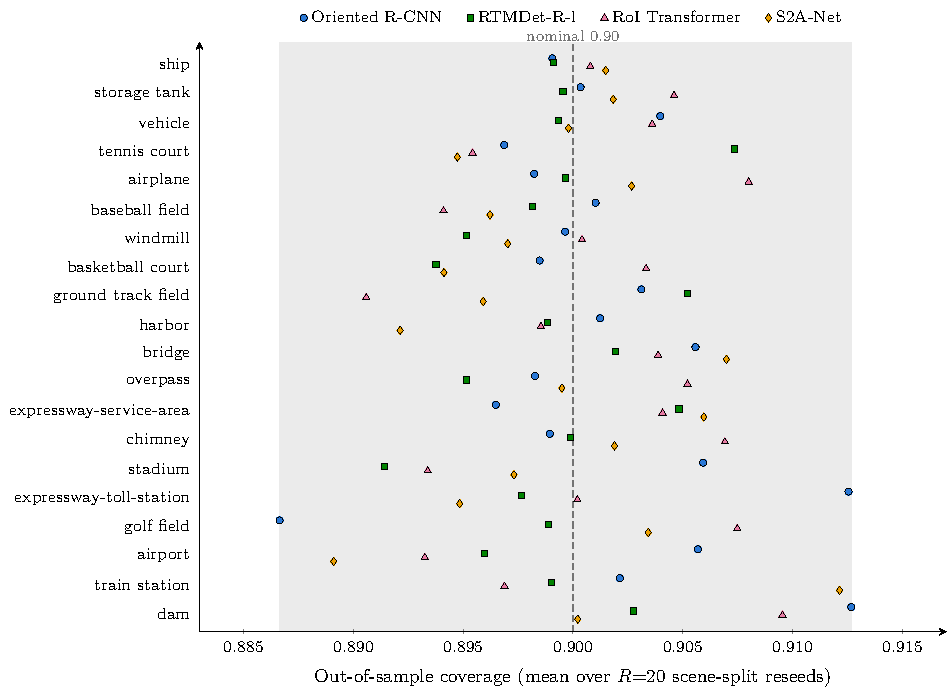
\includegraphics{../figures-src/fig1_diorperclass.pdf}
\caption{The four-cell per-class G1 record in detail ($\alpha=0.10$, nominal $0.90$, $R{=}20$
scene-split reseeds). \textbf{a:} per-class out-of-sample conditional coverage --- all $80$
class$\times$cell points sit within the shaded $\approx1.3$-point band around nominal.
\textbf{b:} the reseed spread behind those means (s.d.\ median $0.020$, max $0.053$).
\textbf{c:} certified GWD radius $\hat q$ vs.\ per-class calibration size: rare classes pay for
nominal coverage with a wider region. \textbf{d:} the G1 certifiability floor
$\alpha_{\min}=1/(n_{\mathrm{cal}}{+}1)$ --- every class clears the frozen $\alpha{=}0.10$ by an
order of magnitude; point colour marks the companion G2 recall verdict (certified vs.\ refused),
separating the two certificates' floors. From the frozen four-cell per-class conditional-coverage
record.}\label{fig:diorperclass}
\end{figure}

\subsection{Training-seed stability of the certificates (HRSC 3-seed arm)}\label{sec:seedvar}
% source: hrsc_seedcells_2026-07-14/SEED-VARIANCE-DIGEST.md (seeds 1-2 certified via cert_cell.sh on the pulled
% detections); seed 0 = configA_cert_2026-07-14/hrsc_{orcnn,rtmdet}/ (the Config-A cells, NOT recomputed).
% All alpha=0.10 (nominal 0.90), GWD score, frozen pipeline. Post-hoc/exploratory Config-B arm.
As a post-hoc, exploratory Config-B arm (not a preregistered confirmatory family) we retrained the two in-house
HRSC2016-MS detectors under two further training seeds (seeds $1,2$; seed $0$ is the already-certified Config-A
cell above, not recomputed) and re-ran the frozen certification chain on the pulled detections.
Table~\ref{tab:seedvar} reports, per seed, the audited GWD marginal coverage, the matched-true-positive count,
the out-of-sample $R{=}20$ recalibration, and the G2 refusal status.

\begin{table}[t]\centering\small
\caption{HRSC 3-seed arm (post-hoc/exploratory Config-B): per-seed certification quantities at $\alpha=0.10$
(nominal $0.90$), GWD score, same frozen pipeline. Audited marginal coverage (point $[$CI$]$), matched
true-positive count, out-of-sample $R{=}20$ recalibration (mean $[\min,\max]$ over $20$ scene reseeds), and G2
refusal status. Seed $0$ is the already-certified Config-A cell (not recomputed); seeds $1,2$ are added
here.}\label{tab:seedvar}
% source: hrsc_seedcells_2026-07-14/SEED-VARIANCE-DIGEST.md (audit_gwd.json / r20_coverage.json / recall.json)
\begin{tabular}{llcccc}
\toprule
Detector & seed & audited GWD coverage $[$CI$]$ & $n_{\mathrm{TP}}$ & $R{=}20$ mean $[\min,\max]$ & G2 \\
\midrule
Oriented R-CNN & $0$ & $0.9011$ $[0.8798,0.9201]$ & $799$ & $0.8989$ $[0.8528,0.9500]$ & refused (power floor) \\
Oriented R-CNN & $1$ & $0.9023$ $[0.8803,0.9228]$ & $727$ & $0.8982$ $[0.8414,0.9360]$ & refused (power floor) \\
Oriented R-CNN & $2$ & $0.9024$ $[0.8780,0.9246]$ & $758$ & $0.9005$ $[0.8249,0.9545]$ & refused (power floor) \\
RTMDet-R       & $0$ & $0.9015$ $[0.8760,0.9227]$ & $670$ & $0.9085$ $[0.8659,0.9568]$ & refused (power floor) \\
RTMDet-R       & $1$ & $0.9016$ $[0.8799,0.9235]$ & $630$ & $0.9113$ $[0.8839,0.9402]$ & refused (power floor) \\
RTMDet-R       & $2$ & $0.9023$ $[0.8796,0.9232]$ & $737$ & $0.8903$ $[0.8444,0.9311]$ & refused (power floor) \\
\bottomrule
\end{tabular}
\end{table}

Three observations, each scoped to what the arm supports. (a) Coverage lands at nominal for every seed
--- as split-conformal calibration guarantees under exchangeability, not as a nontrivial stability finding:
the audited GWD coverage sits within $0.0013$ of a common value across seeds (Oriented R-CNN
$0.9011$--$0.9024$; RTMDet-R $0.9015$--$0.9023$), i.e.\ no seed-driven exchangeability breakdown occurred.
Split conformal pins the marginal coverage by construction, so this confirms the pipeline rather than
discovering a nontrivial stability. (b) The seed-sensitive quantity is the region scale.
% source: hrsc_seedcells_2026-07-14/QHAT-SPREAD.md + extract_qhat_spread.py (q_hat_across_repeats.mean over the six r20_coverage.json)
The conformal quantile $\hat q$ (the GWD nonconformity radius, in Gaussian--Wasserstein score units)
does vary with the training seed, and unevenly across detectors: the per-seed mean $\hat q$ (over the
$R{=}20$ reseeds) moves only $1.5\%$ for Oriented R-CNN ($39.57$--$40.17$) but $\approx12\%$ for RTMDet-R
($48.23$--$54.26$), so it is the certified region's size, not its coverage, that carries the
training-seed variation. The six out-of-sample $R{=}20$ coverage means all straddle nominal
($0.8903$--$0.9113$), with RTMDet-R's wider across-seed spread ($0.021$) inside each cell's own reshuffle
range (per-cell $[\min,\max]$ spans $\approx0.06$--$0.13$). (c) Refusal is seed-stable: the G2 LTT-HB power-floor refusal
($n_{\mathrm{img}}=440$, below the floor) fires identically in all six cells, so refusal behavior does not
flicker with training randomness. The matched-true-positive counts vary with seed ($630$--$799$) because the
detection sets differ --- the expected detector-side variation the certification wraps, not a pipeline
instability. (Multi-seed DIOR-R detector-depth cells are left to future work.)

\subsection{Preregistered head-to-head: the Holm-8 family (demoted to descriptive)}\label{sec:holm8}
% source: holm8_2026-07-12/holm8_result.json (frozen family per SIGN-OFF-RECORD-2026-07-11;
% protocol: one 40/20/40 cal/match/eval scene split per cell, seed 0; both scores calibrated
% on the SAME matching split at alpha=0.10; paired per-class set sizes on the held-out eval
% split; class-blocked bootstrap CI + sign-flip permutation p; one-sided H1 GWD < baseline.
% DEGENERACY (verified 2026-07-12): pooled calibration => 1 set-size scalar per cell =>
% per-pair permutation p deterministic at 1/2001, bootstrap CI zero-width, effective n=1.
% See holm8_run.py docstring + holm8_2026-07-12/holm8_r20_exploratory.json (R=20 robustness).
\textbf{Preregistered result (descriptive).} The preregistered family --- $2$ baseline contrasts (naive
coordinate-wise + Bonferroni; axis-aligned hull) $\times$ $2$ detectors $\times$ $2$ datasets $= 8$
one-sided tests (H1: GWD region strictly smaller) --- was executed exactly as frozen under the signed freeze
% freeze record: SIGN-OFF-RECORD-2026-07-11
on a single frozen $40/20/40$ cal/match/eval scene split
(split-seed $0$) per cell; the $R{=}20$ across-split robustness below is a separate, exploratory
analysis. GWD is strictly smaller in all $8$ of $8$ cells. We report this as a preregistered
descriptive outcome, not statistical confirmation: as detailed next the single-split test is
structurally degenerate, so the nominal Holm-adjusted $p=0.004$ is an artifact of the $1/2001$ permutation
floor and carries no evidence strength. The eval-split region-size ratios (GWD $\div$ baseline; ``region size'' here $=$ the
$(cx,cy)$-slice area, $\pi\hat q^2$ for GWD and $4\hat q_{cx}\hat q_{cy}$ for the union-bound baselines
--- a coverage-region slice, not a calibrated marginal interval; see \S\ref{sec:methods}) of
$0.67$/$0.86$ (RTMDet--DOTA, vs.\ naive/hull), $0.60$/$0.78$ (ORCNN--DOTA), $0.33$/$0.48$
(ORCNN--DIOR-R), and $0.40$/$0.59$ (RTMDet--DIOR-R): GWD is strictly smaller in every cell.

\textbf{Degeneracy disclosure --- the $p$-values carry no evidence strength.} Under the frozen protocol
both constructions are calibrated with pooled split-conformal (one marginal cell, no Mondrian
grouping) --- not the per-class Mondrian calibration of the shipped G1
certificate (\S\ref{sec:results}), a deliberate mismatch we flag here. (The contrast also pooled all
matched true positives without excluding square-stratum detections; the design's square-vacuity rule
guards the angular set, not this center-localization $(cx,cy)$ slice, so the effect on the
area metric here is limited.) Pooled calibration makes each
construction's region-size a single scalar per cell: $\pi\hat q^2$ and $4\hat q_{cx}\hat q_{cy}$
are functions of scalar quantiles only, so every detection in a cell carries the identical set
size (we re-verified $1$ unique value over all $20$k--$40$k eval pairs per cell; e.g.\ ORCNN--DOTA GWD
$126.6$, naive $212.5$, hull $162.3$\,px$^2$). The preregistered per-pair machinery is therefore
degenerate: every per-pair log-ratio equals the same negative constant, so the class-blocked
bootstrap CI is zero-width and the sign-flip permutation $p$ is deterministic at the
$1/(n_{\mathrm{perm}}{+}1)=1/2001$ floor for any negative effect, independent of magnitude; the
effective sample size is $1$ (a pair of scalars from one split), not the $20$k--$40$k pairs.
The preregistered test thus certifies only the per-split deterministic inequality
$\pi\hat q_{\mathrm{GWD}}^2 < 4\hat q_{cx}\hat q_{cy}$ on the frozen split; its substantive content is
the effect size (the ratios above), not the $p$-values, and ``$8/8$ at the $p$-floor'' is
not eight independent strong rejections. This inequality is moreover close to analytic: the
union-bound (Bonferroni) baselines over-cover by construction at any fixed nominal $\alpha$, so at matched
nominal level their $(cx,cy)$ box is predictably larger than a near-nominal ball --- the ``$8/8$ smaller''
direction largely reflects that structural Bonferroni looseness, not a data-driven margin. The
coverage-matched ablation below is precisely what removes it.

\textbf{Across-split sensitivity of the nominal-level contrast ($R{=}20$; not preregistered).} We recompute
the per-split GWD and baseline region sizes on the same $R{=}20$ scene splits as the G1 coverage headline
% across-split recompute script: holm8_r20_exploratory.py
(split-seed $=$ repeat index), to check how the frozen single-split nominal-level ratio varies by
realization. The direction is stable: GWD's region is smaller on all $20$ of $20$ splits in every one
of the $8$ cells, no split's ratio crosses $1$, and the worst single split anywhere is $0.974$
(RTMDet--DOTA vs.\ hull). Table~\ref{tab:r20holm} reports per-cell mean and $[\min,\max]$ ratios.
We attach no $p$-value to this $20/20$ count: the split procedure reshuffles one fixed scene
set, so the $20$ splits are dependent, overlapping partitions, not $20$ independent draws --- an exact sign
test would treat them as independent and materially overstate the evidence. We therefore read this only as a
split-sensitivity range of the (still descriptive) frozen nominal-level contrast, which it corroborates and
nowhere contradicts. Crucially, this analysis (like the frozen family) compares at matched nominal
$\alpha$, where the baselines over-cover; the coverage-matched ablation next is what tests the efficiency
claim on a coverage-fair footing, and is our primary quantitative support for it.

\begin{table}[t]\centering\small
\caption{Across-split sensitivity ($R{=}20$, not the preregistered Holm-8) of the
GWD-vs-baseline region-size ratio at matched nominal $\alpha$ (GWD $\div$ baseline; ${<}1$ favors
GWD). Per cell: mean and $[\min,\max]$ over $20$ scene splits (split-seed $=$ repeat index, same protocol as
the G1 headline) and the count of splits with GWD smaller. The $20$ splits reshuffle one fixed scene set
(dependent), so no $p$-value is attached; every split favors GWD and no ratio crosses $1$. These
nominal-level ratios are re-assessed on a coverage-fair footing in Table~\ref{tab:covmatched}.}
\label{tab:r20holm}
\begin{tabular}{llccc}
\toprule
Cell & Baseline & mean ratio & $[\min,\max]$ & GWD smaller \\
\midrule
RTMDet--DOTA   & naive & $0.597$ & $[0.519,0.791]$ & $20/20$ \\
RTMDet--DOTA   & hull  & $0.773$ & $[0.687,0.974]$ & $20/20$ \\
ORCNN--DOTA    & naive & $0.573$ & $[0.468,0.683]$ & $20/20$ \\
ORCNN--DOTA    & hull  & $0.746$ & $[0.635,0.876]$ & $20/20$ \\
ORCNN--DIOR-R  & naive & $0.342$ & $[0.307,0.395]$ & $20/20$ \\
ORCNN--DIOR-R  & hull  & $0.493$ & $[0.460,0.567]$ & $20/20$ \\
RTMDet--DIOR-R & naive & $0.381$ & $[0.358,0.431]$ & $20/20$ \\
RTMDet--DIOR-R & hull  & $0.549$ & $[0.505,0.625]$ & $20/20$ \\
\bottomrule
\end{tabular}
% source: holm8_2026-07-12/holm8_r20_exploratory.json (all cells: n_splits_gwd_smaller=20, any_ratio_crosses_one=false)
\end{table}

\textbf{Coverage-matched ablation --- the efficiency claim on a coverage-fair footing.} The contrasts
above equalize the nominal $\alpha=0.10$, not realized coverage. At that level GWD attains
close-to-nominal eval coverage ($R{=}20$ mean $0.883$ on DOTA and $0.899$ on DIOR-R, consistent with the
G1 headline), while the union-bound baselines over-cover --- $R{=}20$ mean realized coverage
$0.915$--$0.948$ across cells --- so part of the nominal size gap is the price of baseline over-coverage.
We therefore run the coverage-matched ablation the previous draft deferred: holding GWD at $\alpha=0.10$,
we re-tune each baseline to a level $\alpha'$ at which its realized eval coverage matches GWD's on
the same split, then compare $(cx,cy)$-slice areas (Table~\ref{tab:covmatched}; frozen split and $R{=}20$
range, realized coverage matched to within $\le 0.0002$).
% source: coverage_matched_2026-07-13/results.json (post-hoc, coverage-fair; not preregistered/confirmatory)
Most of the nominal advantage does not survive. Against the like-for-like naive Bonferroni
baseline --- which, like GWD, certifies the full $5$-DOF oriented box --- GWD stays smaller on DIOR-R across
all four cross-family detectors now certified there (\S\ref{sec:configB}): $\approx0.79\times$ ORCNN,
$\approx0.83\times$ RTMDet, $\approx0.76\times$ RoI Transformer, $\approx0.85\times$ S2A-Net (range
$0.76$--$0.85\times$; smaller on all $20/20$ splits in every one of the four cells),
but on DOTA it is a wash (mean $\approx0.93$, only $12/20$ splits favor GWD, the range spanning
$1$). Against the axis-aligned hull, GWD is larger at matched coverage in every cell run under this
ablation, now six in total ($1.46$--$1.76\times$ the four original cells; $1.66\times$ S2A-Net and
$1.75\times$ RoI Transformer, both within the same band): the nominal hull advantage was over-coverage
plus the hull certifying only
the coarser $4$-DOF axis-aligned envelope (it drops the angle), so its center footprint is tighter at
matched marginal coverage --- a representational caveat, not a GWD defect. At the pooled level the
coverage-fair advantage is narrow: GWD is $\approx0.8\times$ the like-for-like naive oriented-box region
on DIOR-R (all four detectors, every split), a wash on DOTA, and larger than the hull everywhere; but this
pooled view averages over object shape, and conditioning on it (next, Table~\ref{tab:regime}; the
regime-conditional analysis below is not re-run on the two Config-B DIOR-R cells) shows that,
within each of the four frozen cells, the naive-baseline advantage is larger on the more elongated
objects --- a descriptive within-cell pattern, not a mechanism. This ablation is post-hoc but coverage-fair, and is
not confirmatory (no preregistration claim). The premise-death branch of C2 did not fire, and the
paper's correctness contributions (seam-continuity, square-safety, the coupled G1/G2 guarantees) do not
rest on the efficiency margin. Figure~\ref{fig:covmatched} plots the per-cell coverage-matched ratio
against both baselines directly, with the $R{=}20$ range and parity ($\mathrm{ratio}=1$) marked.

\begin{table}[t]\centering\small
\caption{Coverage-matched efficiency ablation (post-hoc, coverage-fair; not preregistered).
Region-size ratio (GWD $\div$ baseline; ${<}1$ favors GWD) with each baseline re-tuned to GWD's realized
eval coverage. Columns: the nominal-$\alpha$ ratio (Table~\ref{tab:r20holm} for the four original cells; for
the two Config-B DIOR-R cells, not part of that preregistered family, this ablation's own $R{=}20$
nominal-$\alpha$ mean) and the coverage-matched ratio
($R{=}20$ mean $[\min,\max]$), plus splits with GWD smaller. The naive baseline certifies the full oriented
box (like GWD); the hull certifies only the coarser axis-aligned envelope. From the coverage-matched
records.}
\label{tab:covmatched}
% source: coverage_matched_2026-07-13/results.json (cells[].ratio_nominal / per_split_ratio_matched); RoI-Trans/S2A-Net rows from
% coverage_matched_configB_ext_2026-07-15/results.json (identical protocol, parent helpers reused verbatim, g1_calibrate cross-check re-verified)
\begin{tabular}{llccc}
\toprule
Cell & Baseline & nominal & matched $[\min,\max]$ & GWD smaller \\
\midrule
RTMDet--DOTA   & naive & $0.60$ & $0.93$ $[0.47,1.26]$ & $12/20$ \\
RTMDet--DOTA   & hull  & $0.77$ & $1.48$ $[1.36,1.63]$ & $0/20$ \\
ORCNN--DOTA    & naive & $0.57$ & $0.93$ $[0.42,1.23]$ & $12/20$ \\
ORCNN--DOTA    & hull  & $0.75$ & $1.46$ $[1.34,1.61]$ & $0/20$ \\
ORCNN--DIOR-R  & naive & $0.34$ & $0.79$ $[0.67,0.89]$ & $20/20$ \\
ORCNN--DIOR-R  & hull  & $0.49$ & $1.76$ $[1.65,1.81]$ & $0/20$ \\
RTMDet--DIOR-R & naive & $0.38$ & $0.83$ $[0.74,0.92]$ & $20/20$ \\
RTMDet--DIOR-R & hull  & $0.55$ & $1.70$ $[1.63,1.82]$ & $0/20$ \\
RoI-Trans--DIOR-R & naive & $0.33$ & $0.76$ $[0.62,0.86]$ & $20/20$ \\
RoI-Trans--DIOR-R & hull  & $0.47$ & $1.75$ $[1.67,1.81]$ & $0/20$ \\
S2A-Net--DIOR-R   & naive & $0.38$ & $0.85$ $[0.74,0.97]$ & $20/20$ \\
S2A-Net--DIOR-R   & hull  & $0.54$ & $1.66$ $[1.56,1.72]$ & $0/20$ \\
\bottomrule
\end{tabular}
\end{table}

% source: figures-src/fig2_covmatched.pdf, rebuilt by figures-src/make_fig2_covmatched.py <-
% coverage_matched_2026-07-13/results.json + coverage_matched_configB_ext_2026-07-15/results.json +
% nondegenerate_perclass_2026-07-26/results.json (verbatim; no recomputed statistics)
\begin{figure}[t]\centering
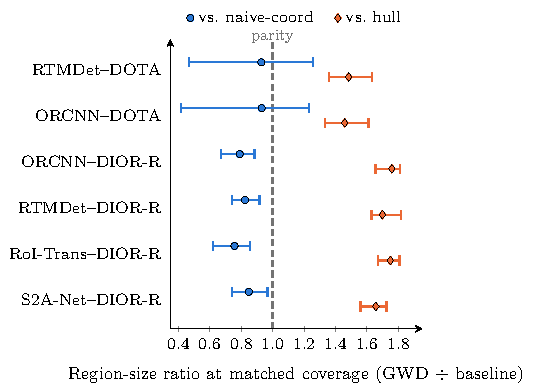
\includegraphics{../figures-src/fig2_covmatched.pdf}
\caption{The coverage-matched efficiency test in full. \textbf{a:} per-cell region-size ratio
(GWD $\div$ baseline; ${<}1$ favors GWD) at realized coverage matched to the GWD certificate,
$R{=}20$ mean with $[\min,\max]$; all four DIOR-R cells sit below parity against the naive
baseline, both DOTA cells straddle it, every cell sits above the hull.
\textbf{b:} all $240$ per-split ratios --- the verdict is not a mean artifact ($104/240$ splits
below parity, cell-dependent). \textbf{c:} the coverage-matching mechanism itself: baseline
$\alpha'$ per cell vs.\ the frozen $\alpha{=}0.10$ line GWD is held to. \textbf{d:} the $180$
class-level non-degenerate cells sorted by area reduction against the best baseline; three carry
CIs excluding zero and none survives Holm ($n_{\mathrm{reject\ Holm}}{=}0$) --- the powerless
test reported as such, not amended. From the frozen coverage-matched and per-class
records.}\label{fig:covmatched}
\end{figure}

\textbf{Within each frozen cell, the coverage-fair naive-baseline advantage is larger on more elongated objects (descriptive).}
% source: coverage_matched_regime_2026-07-13/results.json (regime rows; regression_guard.passed=true, max_abs_diff=0.0 vs parent coverage_matched_2026-07-13)
The pooled ratios above average over object shape, which hides the mechanism. Repeating the
coverage-matched comparison conditioned on the matched ground-truth box's aspect ratio
$\mathrm{AR}=\max(w,h)/\min(w,h)$ --- a property of the ground-truth object, computed without
reference to the certified region, so the strata are not circular, and reusing the parent's per-split
calibration verbatim (the unconditioned ``all'' regime reproduces Table~\ref{tab:covmatched}
bit-for-bit; regression-guarded) --- resolves the pooled numbers into a monotone within-cell trend across
aspect-ratio strata (Table~\ref{tab:regime}). Against the like-for-like naive per-coordinate baseline, at realized coverage
matched to $\le 0.0004$ in every regime, GWD's $(cx,cy)$ region is smaller for elongated
objects ($\mathrm{AR}\ge3$) in all four original cells ($0.74$--$0.87\times$), while for compact
objects ($\mathrm{AR}<3$) it is a wash-to-slight-loss ($0.97$--$1.08\times$, the slight loss confined to
DOTA). A per-cell median split (balanced halves, cut $\approx2.2$--$2.5$) gives the same direction in all
four original cells and sharpens it on DIOR-R, where the more-elongated half reaches $0.59$--$0.65\times$ against
$\approx1.02\times$ on the compact half. This explains the DOTA ``wash'' ($\approx0.93$) rather
than explaining it away: it is the average of a genuine elongated-object win and a slight compact-object
loss, not evidence that the angle-aware region is never sharper --- within these four frozen cells the
efficiency advantage is concentrated on the more elongated objects. We report this as a description of these
four cells, not as a mechanism: HRSC2016-MS, an all-elongated population (eval frac $\mathrm{AR}\ge3$
$0.90$/$0.93$), landed at pooled coverage-matched ratios $1.2413$/$1.0198$ --- outside the four cells'
elongated band ($0.74$--$0.87\times$) and in the wrong direction --- so the within-cell pattern is descriptive
only and did not survive its one out-of-sample test (\S\ref{sec:configA}).

Two scope limits bound the claim honestly. First, this is specifically a repair versus the naive
per-coordinate baseline: against the axis-aligned hull GWD is larger in every regime
($1.4$--$1.8\times$) with no elongation gradient (elongated $\ge$ compact in $3/4$ cells), so the
advantage is not ``smaller than the hull.'' Second, the between-dataset pattern is not an
elongation effect: DOTA objects are on average more elongated than DIOR-R (mean AR $2.70$ vs.\
$2.35$), yet GWD wins pooled on DIOR-R and only ties on DOTA, so the DIOR-vs-DOTA gap tracks the DOTA
crop/exchangeability artifact (\S\ref{sec:results}), not shape --- the elongation effect is
within-cell and conditional. Finally, we can now report the outcome of a registered prediction
% source: coverage_matched_regime_2026-07-13/RESULTS.md + hrsc_prefetch_2026-07-13/PREFETCH-RECORD.md (HRSC2016-MS source train+test, n=3611: AR mean 5.22, 82% AR>=3; logged pre-run 2026-07-13);
% OUTCOME: configA_regime_extend_2026-07-14/results.json (verdict REVERSED: HRSC pooled ratios 1.2413 orcnn / 1.0198 rtmdet, both >=1)
(logged $2026$-$07$-$13$, before the Config-A box run) for the staged third-dataset arm: because
HRSC2016-MS ships (single-class; source mean AR $5.22$, $82\%$ at $\mathrm{AR}\ge3$) lie almost entirely in
the elongated regime, their pooled coverage-matched ratio versus naive-coord was predicted to be the
most decisive GWD win of any cell (low-$0.7\times$ or below); a wash there would falsify the elongation
mechanism. The prediction is reversed. The realized HRSC pooled ratios are $1.2413$ (Oriented
R-CNN) and $1.0198$ (RTMDet-R) --- both $\ge 1.0$ (mean $1.1305$): GWD's matched-coverage region is
larger than naive-coord's on the most elongated dataset. The two DOTA zoo cells on the same dataset
and eval set add strong detector-dependence in the same direction ($1.6618$ RoI Transformer vs.\ $0.7056$
Oriented RepPoints). We therefore withdraw any cross-dataset elongation-mechanism claim: the elongation
effect does not transfer between datasets or detectors. What survives is the within-cell
elongation pattern on the four original frozen cells (Table~\ref{tab:regime}), reported as a descriptive,
post-hoc observation only; and, as on every earlier cell, GWD never beats the axis-aligned hull (the new
cells give $1.30$--$2.44\times$: HRSC $1.82$/$1.30$, zoo $2.44$/$1.43$, consistent with the frozen
$1.4$--$1.8\times$). Two population caveats bound this cross-cell reading: HRSC2016-MS has essentially no
compact stratum (eval mean AR $5.63$/$5.95$, frac $\mathrm{AR}\ge3$ $0.90$/$0.93$; its compact regime rows
are skipped for want of a powered split), and the DOTA zoo cells run on a $1093$-image subset whose matched
population is far less elongated (mean AR $1.27$/$1.47$, frac $\mathrm{AR}\ge3$ $0$/$0.039$) than the
frozen DOTA cells (mean AR $\approx2.7$, frac $\approx0.29$--$0.30$), so the zoo ratios are detector-breadth
evidence, not a third elongation datapoint.

\textbf{Confinement of the coverage-fair efficiency claim.} Netted out, the coverage-fair naive-baseline size
advantage is currently demonstrated on one of the three datasets: GWD is $\approx0.76$--$0.85\times$ the
like-for-like naive region on DIOR-R (all four detectors --- ORCNN, RTMDet, RoI Transformer, S2A-Net --- all
$20/20$ splits), a wash on DOTA
($\approx0.93$), and reversed on HRSC2016-MS ($1.2413$/$1.0198$, both $\ge1.0$). The DOTA wash was
attributed to a crop/exchangeability artifact of DOTA's overlapping tiles (\S\ref{sec:results},
\S\ref{sec:limitations}), but that account cannot rescue the claim's generality: HRSC2016-MS is certified
single-tile (scene $=$ image, uncropped, $453$ whole test images resized in place), so its reversal
on the most elongated dataset cannot be a crop artifact. The efficiency advantage is therefore reported as
DIOR-R-specific, not general.

\begin{table}[t]\centering\small
\caption{Regime-conditional coverage-matched efficiency versus the naive per-coordinate
Bonferroni baseline (post-hoc, coverage-fair; not preregistered). Ratio GWD $\div$ naive of the
$(cx,cy)$-slice area (${<}1$ favors GWD), conditioned on the matched ground-truth box aspect ratio
$\mathrm{AR}=\max(w,h)/\min(w,h)$; realized coverage matched to $\le 0.0004$ in every regime.
For the four original frozen cells the ``all'' column reproduces Table~\ref{tab:covmatched}'s pooled
ratio bit-for-bit (regression-guarded), and elongated objects favor GWD while compact objects are a
wash-to-slight-loss. The out-of-sample Config-A extension cells (HRSC2016-MS, DOTA-v1.0 zoo;
\S\ref{sec:configA}) do not transfer the gradient --- HRSC is $\ge1$ despite being almost all elongated,
and the DOTA-zoo cells are near-all compact (\textemdash{}$=$regime with no powered split). Against the
axis-aligned hull the gradient does not hold (text). From the regime-conditional coverage-matched
records.}\label{tab:regime}
% source: coverage_matched_regime_2026-07-13/results.json (four original cells; rows[].ratio_matched_mean by regime; aspect_ratio_by_cell.{ar_mean,frac_elongated_ge3}; regression_guard.passed=true, max_abs_diff=0.0);
% configA_regime_extend_2026-07-14/results.json (HRSC + zoo rows; rows[].ratio_matched_mean by regime; aspect_ratio_by_cell.{ar_mean,frac_elongated_ge3}; None regimes rendered as --)
\begin{tabular}{lcccc}
\toprule
Cell & AR mean (frac ${\ge}3$) & all & compact (AR${<}3$) & elongated (AR${\ge}3$) \\
\midrule
\multicolumn{5}{l}{Four original frozen cells (within-cell elongation gradient)} \\
RTMDet--DOTA   & $2.69$ ($0.29$) & $0.93$ & $1.03$ & $0.85$ \\
ORCNN--DOTA    & $2.71$ ($0.30$) & $0.93$ & $1.08$ & $0.74$ \\
ORCNN--DIOR-R  & $2.38$ ($0.22$) & $0.79$ & $0.98$ & $0.87$ \\
RTMDet--DIOR-R & $2.34$ ($0.21$) & $0.83$ & $0.97$ & $0.86$ \\
\midrule
\multicolumn{5}{l}{Out-of-sample Config-A extension (gradient does not transfer)} \\
HRSC ORCNN         & $5.63$ ($0.90$) & $1.24$ & \textemdash{} & $1.26$ \\
HRSC RTMDet-R      & $5.95$ ($0.93$) & $1.02$ & \textemdash{} & $0.98$ \\
DOTA RoI Transf.   & $1.27$ ($0.00$) & $1.66$ & $1.66$ & \textemdash{} \\
DOTA RepPoints     & $1.47$ ($0.04$) & $0.71$ & $0.74$ & \textemdash{} \\
\bottomrule
\end{tabular}
\end{table}

\section{Discussion}\label{sec:discussion}
The study is best read as a certification layer for oriented object detectors rather than a new detector architecture. Pattern Recognition reviewers should therefore judge the contribution by whether the layer turns fixed detector outputs into actionable, distribution-free readouts: a center-radius bound, an orientation-extent bound, a rotated-IoU floor, and a separate recall certificate with explicit power-floor refusals. The strongest evidence for that claim is the out-of-sample $R{=}20$ recalibration record: the DIOR-R class certificates survive across detector families, while DOTA and G2 expose the calibration-budget and exchangeability limits instead of being hidden behind a single pooled score.

This separation also explains why negative results are retained as first-class outputs. The DOTA exchangeability warning, the G2 refusals for rare classes, and the degenerate coverage-matched efficiency test are not failures of the submission package; they delimit when the certificates are informative. In a deployment setting, the practical rule is to publish the certificate only for cells whose calibration pool can support the target risk and to report refusal otherwise. The same logic motivates the full-study design below: the present evidence is enough to support the per-class certification interface and its DIOR-R behavior, but cross-dataset claims about angle-aware efficiency require the staged extension rather than extrapolation from the frozen pilot.

\section{Limitations}\label{sec:limitations}
\textbf{Certificate scope (v1).} G1 is conditional on detection: it certifies localization for matched
true positives, not whether an object is detected (G2's separate guarantee). The certified object is the
GWD-ball in Gaussian-Wasserstein space, not an IoU level-set (Methods); its per-parameter envelope
over-covers and is not a set of calibrated coordinate intervals. Guarantees are valid for the calibration
distribution only; the tool prints a recalibrate-on-drift caveat.

\textbf{Scale and the DOTA under-coverage.} The out-of-sample DOTA coverage ($0.888$) sits $\approx1.2$ points
below nominal; we attribute this to residual within-scene correlation in DOTA's overlapping crops (the same
detector covers at nominal on single-tile DIOR-R), but a weighted/adaptive conformal remedy for the crop
structure is future work. The $R{=}20$ per-split spread bounds how much this varies by realization.

\textbf{Frozen-checkpoint variance.} The DOTA detector is a frozen published checkpoint (no training-seed
variance; variance is over split repeats). The DIOR-R and HRSC2016-MS detectors are trained in house; for
HRSC2016-MS a post-hoc $3$-seed arm (\S\ref{sec:seedvar}) quantifies training-seed variance: audited coverage
is seed-stable by construction (within-detector spread $\le0.0013$) while the certified region scale $\hat q$
does vary with seed (up to $\approx12\%$ for RTMDet-R), and all four DIOR-R cells remain single-seed
(multi-seed DIOR-R detector variance is future work). The two DOTA zoo detectors (RoI Transformer, Oriented
RepPoints, \S\ref{sec:configA}) are frozen published checkpoints; note that ``RoI Transformer'' therefore
names two distinct trained instances in this paper --- a frozen DOTA-v1.0 zoo checkpoint (\S\ref{sec:configA})
and an independently in-house-trained DIOR-R model (\S\ref{sec:configB}) --- never the same weights certified
twice.

\textbf{Statistical significance and scoop currency.} The regime-conditional under-coverage contrast is
descriptive here; the preregistered Holm set-size head-to-head ran under the signed freeze and is reported in
\S\ref{sec:holm8}, where the frozen single-split family is demoted to a preregistered descriptive
outcome (GWD smaller in $8/8$ cells at nominal $\alpha$) --- structurally degenerate, so not presented as
confirmatory and not amended. Because that $8/8$ is at matched nominal $\alpha$, where the baselines
over-cover, our primary quantitative characterization of efficiency is the post-hoc, coverage-fair
coverage-matched ablation (\S\ref{sec:holm8}, Tables~\ref{tab:covmatched}--\ref{tab:regime}): it shows the
size advantage is largely baseline over-coverage, and that the residual advantage over the like-for-like
naive baseline is, descriptively and within each of the four original cells, larger on more elongated
objects --- GWD's region is smaller for elongated objects (aspect ratio $\ge3$) in all four original cells
($0.74$--$0.87\times$) and a wash-to-slight-loss for compact ones --- while against the axis-aligned hull GWD
is larger in every regime. This gradient is now
scoped to a within-cell, descriptive observation: the falsifiable prediction for the
elongation-dominated HRSC2016-MS ship arm was executed and reversed (\S\ref{sec:configA},
\S\ref{sec:holm8}; HRSC pooled ratios $1.2413$/$1.0198$, both $\ge1.0$), so the elongation mechanism does not
transfer across datasets or detectors and no cross-dataset efficiency claim is made. The $R{=}20$ across-split analysis is reported as
split-sensitivity of the nominal contrast, with no $p$-value (the $20$ splits reshuffle one fixed
scene set and are not independent). The differentiation against EAV-DETR
\citep{eavdetr2026} (\S\ref{sec:related}) rests on its public abstract and code release, its full text being
paywalled. The DIOR-R AOPG mAP reproduction
gate was executed (reproduced test mAP $62.61$ / $68.36$ vs.\ AOPG $64.41$; $\pm0.5$ not met cross-method;
same-method external anchor $64.30$ \citep{ding2026rtoriented}, disclosed).
% source: holm8_2026-07-12/holm8_result.json (frozen family executed, demoted to descriptive);
% AOPG repro executed 2026-07-13 (aopg_repro_2026-07-13/; FAIL vs +-0.5 cross-method, disclosed)

\section{Full-study design}\label{sec:fullstudy}
% source: holm8_2026-07-12/holm8_result.json (Holm-8 family executed as frozen; demoted to descriptive, single-split p degenerate)
The pilot and DIOR-R cells instantiate the G1/G2 arms; the preregistered study adds the $R{=}20$ repeats for
every cell (done for the coverage headline) and the preregistered
Holm family (the paper's only Holm family: $2$ baseline contrasts $\times$ $2$ detectors $\times$ $2$ datasets
$=8$ tests), which ran under the signed freeze and is reported in \S\ref{sec:holm8} (GWD smaller in $8/8$
cells, demoted to a preregistered descriptive outcome; no amendment). The AOPG mAP reproduction gate has now
been executed (\S\ref{sec:results}); no preregistration-gated slot remains. The staged third-dataset
(HRSC2016-MS) arm and the DOTA detector-zoo breadth were executed as the Config-A extension
(\S\ref{sec:configA}); the registered elongation prediction it tested is reported reversed (\S\ref{sec:holm8}).
The cross-family DIOR-R detector-breadth arm (RoI Transformer, S2A-Net) was executed as the Config-B
extension (\S\ref{sec:configB}); both new cells certify at G1 with zero Mondrian refusals.
% AOPG repro executed 2026-07-13 (aopg_repro_2026-07-13/; measured 62.61/68.36 vs AOPG 64.41; FAIL vs +-0.5 cross-method, disclosed)
% Config-A extension executed 2026-07-14 (configA_cert_2026-07-14/, configA_regime_extend_2026-07-14/; HRSC prediction REVERSED)
% Config-B DIOR breadth arm executed 2026-07-15 (configB_cells_2026-07-15/{roi_trans,s2anet}; 0/20 G1 refusals both cells)

\section{Conclusions}\label{sec:conclusions}
This paper set out to give oriented object detection in aerial imagery a distribution-free
reliability layer, and delivers it as actionable per-class certificates: validated out-of-sample on
DIOR-R across four detector architectures with all $20$ classes certified and none refused, and
translated into readouts an operator can act on --- a certified center-offset radius in pixels, an
orientation half-extent in degrees that is tight exactly where orientation is meaningful, and a
per-class rotated-IoU floor. The enabling observation is methodological: the $2$-Wasserstein
distance between box-induced Gaussians is a seam-continuous, square-safe nonconformity score, while
a coordinate-wise angle interval is structurally mis-specified at the $\pm 90^\circ$ seam and at
square boxes (Figure~\ref{fig:seamsquare}). Two companion guarantees bound what the main
certificate does not cover: a Learn-then-Test certified recall bound (G2), and explicit refusal
semantics wherever a stratum's calibration pool cannot support the requested level.

The study's weaknesses are equally concrete. On DOTA-v1.0 the certificate sits $1$--$1.2$ points
below nominal because the standard overlapping-crop pipeline correlates neighbouring evaluations
--- the guarantee's exchangeability premise, not the score, is what breaks; a weighted or
scene-adaptive conformal construction for crop structure is the clear next step. G2 certifies only
classes with large image counts and refuses most classes at realistic per-class support. The
efficiency advantage of the GWD region over naive baselines is established only descriptively ---
the preregistered inferential family is structurally degenerate --- and does not transfer across
datasets (a registered elongation prediction reversed on the HRSC2016-MS arm). Finally, all DIOR-R
detectors are single-seed, and the certified detectors reproduce below their published mAP.

Beyond the crop-structure remedy, future work includes multi-seed detector variance on DIOR-R,
drift-triggered recalibration (the tool already prints a recalibrate-on-drift caveat), and
extending the same certification layer from boxes to instance-segmentation masks. The
\texttt{rotcert} tool, frozen result records, and golden-file-tested CLI accompany the paper.

\section*{Declaration of competing interest}
The author declares that he has no known competing financial interests or personal relationships
that could have appeared to influence the work reported in this paper.

\section*{Funding}
This research did not receive any specific grant from funding agencies in the public, commercial,
or not-for-profit sectors.

\section*{CRediT authorship contribution statement}
\textbf{Zeyu Fu:} Conceptualization, Methodology, Software, Validation, Formal analysis,
Investigation, Data curation, Writing -- original draft, Writing -- review \& editing,
Visualization, Project administration.

\section*{Declaration of generative AI and AI-assisted technologies in the manuscript preparation process}
During the preparation of this work the author used Claude (Anthropic) in order to assist with
code development, experiment orchestration, and language editing. After using this tool, the
author reviewed and edited the content as needed and takes full responsibility for the content of
the published article.

\section*{Data and Code Availability}
% frozen records accompanying the paper: holm8_result.json (frozen head-to-head),
% holm8_r20_exploratory.json (across-split analysis); provenance/git_dirty stamped in-record.
DOTA-v1.0 (public; val GT used, test server untouched) and DIOR-R (public; in-house-trained detectors under
Apache-2.0 mmrotate). The \texttt{rotcert} tool (numpy/scipy/shapely only; no torch/mmrotate in the certifier)
and all frozen result records (DOTA pilot, DIOR-R Oriented R-CNN and RTMDet-R-l, the out-of-sample $R{=}20$
coverage, the naive regime audits, the frozen preregistered head-to-head record, the across-split analysis
record, and the coverage-matched ablation record) accompany the paper; the CLI is golden-file-tested against
these records. The \texttt{rotcert} tool and all frozen result records are archived at Zenodo (DOI:
10.5281/zenodo.21392293) with a rotcert-scoped public release of the development tree and records at
\url{https://github.com/PeterPonyu/rotcert}, matching the scoped public-release pattern used for
\texttt{PeterPonyu/asr-gate} and \texttt{PeterPonyu/inspect-gate}. The surrounding private
\texttt{PeterPonyu/reliability-commons} monorepo is not published wholesale because it contains
other manuscripts and submission materials.
Provenance note: the
frozen head-to-head record was written with a dirty working tree (uncommitted changes present when the
preregistered family ran); the exact script and environment are stamped in the record's own provenance
metadata. Detector weights are frozen published checkpoints (DOTA) or in-house-trained (DIOR-R, redistribution
subject to the DIOR-R license review; result-records-only if rehosting is barred). The Config-A extension
records (four new G1 certification cells on HRSC2016-MS and the DOTA detector zoo, their $R{=}20$
recalibration, the G2 power-floor refusals, and the reversed registered-prediction verdict) accompany the
paper as well, as do the Config-B extension records (two new G1 certification cells on DIOR-R --- RoI
Transformer, S2A-Net --- their $R{=}20$ recalibration, G2 status, and the extended four-cell per-class
conditional-coverage record).

\bibliographystyle{plainnat}
\bibliography{refs}

\end{document}
